\documentclass[12pt]{tufte-handout}
%% \documentclass[reqno,12pt]{tufte-book}
%% \usepackage{trace}
%% \documentclass[reqno,12pt]{article}

\usepackage{appendix}

%% \usepackage{csquotes}

\usepackage{amsmath}
\usepackage{setspace}
\numberwithin{equation}{subsection}
\usepackage{amsthm}
\usepackage{amsfonts}

\usepackage{stmaryrd}

%% broken (doesn't work with tufte-handout):
\usepackage{zed-csp}
%% broken:
%% \usepackage{ltcadiz-fam}

\usepackage{fontspec}
%% \usepackage{xltxtra,xunicode}
\defaultfontfeatures{Scale=MatchLowercase}

%% \defaultfontfeatures{Scale=MatchLowercase}
%% \setmainfont[Mapping=tex-text]{Times New Roman}
%% \setsansfont[Mapping=tex-text]{Arial}
%% \setmonofont{Courier}

\setmainfont[Ligatures=TeX]{TeX Gyre Bonum}
\setromanfont[Ligatures=TeX]{TeX Gyre Bonum}
\setsansfont[Ligatures=TeX]{TeX Gyre Adventor}
\setmonofont[Ligatures=TeX]{TeX Gyre Cursor}


%% \setmainfont[Mapping=tex-text]{Minion Pro}
%% \setromanfont[Mapping=tex-text]{Minion Pro}
%% \setsansfont[Mapping=tex-text]{TeX Gyre Heros}

%% Bugfix: see https://code.google.com/p/tufte-latex/issues/detail?id=64
% Set up the spacing using fontspec features
\renewcommand\allcapsspacing[1]{{\addfontfeature{LetterSpace=15}#1}}
\renewcommand\smallcapsspacing[1]{{\addfontfeature{LetterSpace=0.0}#1}}

\usepackage{epigraph}
\setlength{\epigraphwidth}{.8\textwidth}

%% general symbols - degree, etc.
\usepackage{gensymb}

\usepackage [english]{babel}
\usepackage [autostyle, english = american]{csquotes}

\usepackage{mflogo}

\numberwithin{equation}{subsection}

%% nice double-stroke fonts
\usepackage{dsfont}

% Small sections of multiple columns
\usepackage{multicol}

% Provides paragraphs of dummy text
\usepackage{lipsum}

% The following package makes prettier tables.  We're all about the bling!
\usepackage{booktabs}

% The units package provides nice, non-stacked fractions and better spacing
% for units.
\usepackage{units}

\usepackage{xcolor,mdframed}

%\usepackage{geometry}                % See geometry.pdf to learn the layout options. There are lots.
%\geometry{letterpaper}                   % ... or a4paper or a5paper or ...

\usepackage{xfrac}

\usepackage{hyperref}
\hypersetup{
  bookmarks=true,         % show bookmarks bar?
  bookmarksdepth=3,
  unicode=true,          % non-Latin characters in Acrobat’s bookmarks
  pdftoolbar=true,        % show Acrobat’s toolbar?
  pdfmenubar=true,        % show Acrobat’s menu?
  pdffitwindow=false,     % window fit to page when opened
  pdfstartview={FitH},    % fits the width of the page to the window
  pdftitle={The Poetics of Coordinate Space},    % title
  pdfauthor={G. A. Reynolds},     % author
  pdfsubject={Coordinate Space},   % subject of the document
  pdfcreator={G. A. Reynolds},   % creator of the document
  pdfproducer={Producer}, % producer of the document
  pdfkeywords={Coordinate Space} {Graphics}
  pdfnewwindow=true,      % links in new window
  colorlinks=true,       % false: boxed links; true: colored links
  linkcolor=blue,          % color of internal links
  citecolor=blue,        % color of links to bibliography
  filecolor=magenta,      % color of file links
  urlcolor=cyan           % color of external links
}

%% \usepackage[
%% bibstyle=numeric,
%% citestyle=authoryear,
%% hyperref,
%% bibencoding=utf8,
%% backref=true,
%% backend=biber]{biblatex}

%% http://tex.stackexchange.com/questions/66778/citation-alias-with-multibib-and-natbib
%% \makeatletter
%% \def\@mb@citenamelist{cite,citep,citet,citealp,citealt,citepalias,citetalias}
%% \makeatother

%% http://stackoverflow.com/questions/2496599/how-do-i-cite-the-title-of-an-article-in-latex
\defcitealias{z-iso-13568}{ISO 13568:2002 Information technology -- Z formal specification notation --
  Syntax, type system and semantics}

\usepackage{tikz}
\usetikzlibrary{%
  arrows%
  ,calc%
  ,decorations.text%
  ,decorations.pathreplacing%
  ,fadings%
  ,positioning
  ,shapes.geometric%
}

\usepackage{tikz-3dplot}

\usepackage{pgfplots}
\pgfplotsset{height=7cm,compat=1.9}

\usepackage{tkz-euclide}
\usetkzobj{all}

%% prettier integral syms, but broken on miktex
%% \usepackage{esint}


\title{The Poetics of Coordinate Space}
\author{G. A. Reynolds}
%\date{}                                           % Activate to display a given date or no date

%%%%%%%%%%%%%%%%
%% tufte-latex customizations

\makeatletter
\let\runauthor\@author
\let\runtitle\@title
\makeatother

%% running headers
\newcommand{\changefont}{%
  \fontsize{7}{9.5}\selectfont
}
\fancypagestyle{plain}{
  \fancyhead[LO,LE]{\leftmark }
  \fancyhead[RO,RE]{\rightmark}
  \fancyfoot[CO,CE]{\thepage}
  \fancyfoot[LE]{\textsc{\runtitle}}
  \fancyfoot[RO]{\textsc{\runtitle}}
  \renewcommand{\headrulewidth}{0pt}
  \renewcommand{\footrulewidth}{0pt}
}
\pagestyle{plain}

\def\chpcolor{blue!45}
\def\chpcolortxt{blue!60}
\def\sectionfont{\LARGE}

\setcounter{secnumdepth}{2}

\makeatletter
%% Section:
\def\@sectionstrut{\vrule\@width\z@\@height12.5\p@}
\def\@makesectionhead#1{%
  {%\par\vspace{20pt}%
    \parindent -10pt\raggedleft\sectionfont
    %% \colorbox{\chpcolor}{%
    %%   \parbox[t]{90pt}{\color{white}\@sectionstrut\@depth4.5\p@\hfill
    %%     \ifnum\c@secnumdepth>\z@\thesection\fi}%
    %% }%
    \vspace{10pt}%
    \begin{minipage}[t]{\textwidth}%{\dimexpr\textwidth-90pt-2\fboxsep\relax}
      \@sectionstrut\hspace{-15pt}\textit{\textbf\Huge #1}
    \end{minipage}\par
    \vspace{5pt}%
  }
}
%% \def\@makesectionhead#1{%
%%   {\par\vspace{20pt}%
%%    \parindent 0pt\raggedleft\sectionfont
%%    \colorbox{\chpcolor}{%
%%      \parbox[t]{90pt}{\color{white}\@sectionstrut\@depth4.5\p@\hfill
%%        \ifnum\c@secnumdepth>\z@\thesection\fi}%
%%    }%
%%    \begin{minipage}[t]{\dimexpr\textwidth-90pt-2\fboxsep\relax}
%%    \color{\chpcolortxt}\@sectionstrut\hspace{5pt}\textbf{#1}
%%    \end{minipage}\par
%%    \vspace{10pt}%
%%   }
%% }
\def\section{\@afterindentfalse\secdef\@section\@ssection}
\def\@section[#1]#2{%
  \ifnum\c@secnumdepth>\m@ne
  \refstepcounter{section}%
  \addcontentsline{toc}{section}{\protect\numberline{\thesection}#1}%
  \else
  \phantomsection
  \addcontentsline{toc}{section}{#1}%
  \fi
  \sectionmark{#1}%
  \if@twocolumn
  \@topnewpage[\@makesectionhead{#2}]%
  \else
  \@makesectionhead{#2}\@afterheading
  \fi
}
\def\@ssection#1{%
  \if@twocolumn
  \@topnewpage[\@makesectionhead{#1}]%
  \else
  \@makesectionhead{#1}\@afterheading
  \fi
}
\makeatother

%%%%%%%%%%%%%%%%
%% macros

\newenvironment{important}[1][]{%
  \begin{mdframed}[%
      backgroundcolor={red!15}, hidealllines=true,
      skipabove=0.7\baselineskip, skipbelow=0.7\baselineskip,
      splitbottomskip=2pt, splittopskip=4pt, #1]%
    \makebox[0pt]{% ignore the withd of !
      \smash{% ignor the height of !
        \fontsize{32pt}{32pt}\selectfont% make the ! bigger
        \hspace*{-19pt}% move ! to the left
        \raisebox{-2pt}{% move ! up a little
          {\color{red!70!black}\sffamily\bfseries !}% type the bold red !
        }%
      }%
    }%
}{\end{mdframed}}

%% reversed integral sign
\makeatletter
\providecommand*{\curv}{%
  \mathrel{%
    \mathpalette\@curv\int
  }%
}
\newcommand*{\@curv}[2]{%
  \reflectbox{$\m@th#1#2$}%
}
\makeatother



\newtheorem{theorem}{Theorem}
%\newtheorem{cor}{Corollary}
%\newtheorem{lem}{Lemma}
\newtheorem*{defn}{Definition}
%% \theoremstyle{remark}
\newtheorem{remark}{Remark}
\newtheorem*{commentary}{Commentary}
\newtheorem*{todo}{TODO}
\newtheorem{eg}{Example}

\newcommand\cspace{coordinate space}
\newcommand\Cspace{Coordinate space}
\newcommand\CSpace{Coordinate Space}

\newcommand\dspace{design space}
\newcommand\Dspace{Design space}
\newcommand\DSpace{Design Space}

\newcommand\Omg{\(\Omega\)}
\newcommand\sccs{standard cartesian coordinate space}
\newcommand\origin{\((0,0)\)}
\newcommand\ab{\((a,b)\)}
\newcommand\xy{\((x,y)\)}

\newcommand\N{\(\mathds{N}\)}
\newcommand\R{\(\mathds{R}\)}
\newcommand\RR{\(\mathds{R}\times\mathds{R}\)}
\newcommand\Rtwo{\(\mathds{R}^2\)}
\newcommand\Z{\(\mathds{Z}\)}

%%%%%%%%%%%%%%%%%%%%%%%%%%%%%%%%%%%%%%%%%%%%%%%%%%%%%%%%%%%%%%%%
\begin{document}
%% \ifx\traceon\undefined \tracingall \else \traceon \fi

\maketitle

\begin{abstract}
  \begin{center}
    \textit{Abstract}
  \end{center}
  The foundation of any graphics language or system is its coordinate
  system.  Coordinate systems organize space.  Despite my title--a
  play on G. Bachelard's famous \textit{The Poetics of Space}--this is
  a paper on the design and specification of a technical language
  of \cspace{}s.
\end{abstract}

\tableofcontents

\begin{remark}
  To cover: coordinate spaces, axes, transform functions, location
  expression (single points), space transformation expression (all
  points); size, bounding box, mapping to device/viewport space.

  Expressivity:  transform functions v. expressions
\end{remark}

\newpage
%%%%%%%%%%%%%%%%%%%%%%%%%%%%%%%%
\section{Introduction}
\label{sect:intro}

What this is about.  Two things: graphics and languages.  The former
motivates analysis and description of \cspace{}s and graphical
figures; the latter motivates use of formal notations (lambda
calculus and Z) to do so.

Our strategy is as follows.  We model \cspace{}s as a \textit{type}
(symbol: \Omg).  Every type has a carrier set whose elements are
values of that type, so the carrier set of \Omg{} includes all
possible \cspace{}s.  When we combine a \cspace{} and a collection of
geometric \textit{figures} (another type; symbol \(\Gamma\)), we get
another type: \dspace{} (symbol: \(\Delta\)).  The carrier set of
\(\Delta\) thus contains all possible combinations of every \cspace{}
with all possible collections of figures.  It follows that the
operation of ``adding'' a figure to a \dspace{} -- call it the
\textit{inscribe} operation -- is nothing more than a function mapping
a pair of values (one \(\Delta\) value and on \(\Gamma\) value) to
another \(\Delta\) value.

We express this model using the Z formal specification notation.  In
effect, we specify a ``Z toolkit'' that extends the notation to cover
the semantic domain of graphics.  At the moment we use Z because of
its expressive power; it makes it relatively easy to write down
formally correct definitions in an idiom that remains intuitive and
easily understood.  Since Z has a formal semantics, various automated
Z specification checkers are available; at some point in the future we
might try to use one to verify our specification.  But for the moment
our main concern is expressive.

One test of the adequacy of this model is whether it is sufficient to
fully specify the semantics of the TikZ/PGF language.  To our
knowledge, TikZ is the most sophisticated and powerful graphics
language available today.

%%%%%%%%
\subsection{Basic Concepts}

Coordinate space:  unit, axes, etc.  Basic cartesian space.

Expressivity: specification of points in a space v. transformation of
spaces (all points).  No fundamental distinction; a function that can
be used for one can be used for the other.  It's a question of how one
designs the language, what sort of expressiveness it has.

%%%%%%%%
\subsection{\CSpace{}s}
\label{subs:cskinds}

There are two basic kinds of \cspace: discrete and continuous.

A language for continous space will be more expressive than a language
for discrete space.  An expression like \((\pi,\pi)\) is meaningful
for continuous spaces, but not for discrete spaces.  The reason is
simple: they have distinct ``carrier sets''.  The carrier set for a
discrete space is \(\nat\cross\nat\); for continuous spaces, \RR{}.

There are also several types of continuous \cspace.  Rectilinear
(cartesian) spaces are distinct from polar spaces, for example.
Points in both have the same type (\RR), and both contain the same set
of points of this type, but their meanings differ.  An expression like
\((1,1)\) denotes the same pair of real numbers in each space, but
maps to different (spatial) locations.

\begin{description}
\item [Linear]
\item [Polar]
\item [Cylindrical]  Blah blabla bla

  %% see http://en.wikipedia.org/wiki/Cylindrical_coordinate_system
  \begin{marginfigure}[-2in]%
    %% tikz-3dplot manual p. 26-27
    \tdplotsetmaincoords{60}{110}
    %
    \pgfmathsetmacro{\rvec}{1}
    \pgfmathsetmacro{\thetavec}{30}
    \pgfmathsetmacro{\phivec}{60}
    %
    \begin{tikzpicture}[scale=4,tdplot_main_coords]
      \coordinate (O) at (0,0,0);
      \draw[thick,->] (0,0,0) -- (.8,0,0) node[anchor=north east]{$x$};
      \draw[thick,->] (0,0,0) -- (0,.8,0) node[anchor=north west]{$y$};
      \draw[thick,->] (0,0,0) -- (0,0,1) node[anchor=south]{$z$};
      \tdplotsetcoord{P}{\rvec}{\thetavec}{\phivec}
      %% \draw[-stealth] (O) -- (P) node[left,pos=.7] {$r$}
      \fill[red] (P) circle (.5pt)  node[right] {$(\rho,\phi,z)$};
      \draw[dashed] (O) -- (Pxy);
      \draw[dashed] (Pz) -- (P);
      \draw[color=red] (P) -- (Pxy);
      %% FIXME: get coords right
      \draw[dashed,color=gray] (Pz) -- (.6,0,.9);
      \draw[dashed,color=gray] (.6,0,.9) -- (.5,0,0);

      \draw[color=red,thick] (O) -- (.5,0,0);
      \tdplotdrawarc[dashed,color=gray]{(Pz)}{0.5}{0}{\phivec}{anchor=north}{}
      \tdplotdrawarc[-latex,color=red,thick]{(O)}{0.5}{0}{\phivec}{anchor=north}{$\phi$}
      \tdplotsetthetaplanecoords{\phivec}
      %% \tdplotdrawarc[-latex,tdplot_rotated_coords]{(0,0,0)}{0.2}{0}%
      %%               {\thetavec}{above left=0pt and -8pt}{$\phi$}
      %% \tdplotsetrotatedcoords{\phivec}{\thetavec}{0}
      %% \tdplotsetrotatedcoordsorigin{(P)}
    \end{tikzpicture}
    \caption{Point in cylindrical coordinate space.}
  \end{marginfigure}

\item [Spherical]

  \begin{marginfigure}
    %% tikz-3dplot manual p. 26-27
    \tdplotsetmaincoords{60}{110}
    %
    \pgfmathsetmacro{\rvec}{.8}
    \pgfmathsetmacro{\thetavec}{30}
    \pgfmathsetmacro{\phivec}{60}
    %
    \begin{tikzpicture}[scale=4,tdplot_main_coords]
      \coordinate (O) at (0,0,0);
      \draw[thick,->] (0,0,0) -- (.5,0,0) node[anchor=north east]{$x$};
      \draw[thick,->] (0,0,0) -- (0,.5,0) node[anchor=north west]{$y$};
      \draw[thick,->] (0,0,0) -- (0,0,.8) node[anchor=south]{$z$};
      \tdplotsetcoord{P}{\rvec}{\thetavec}{\phivec}
      \draw (O) -- (P) node[left,pos=.7] {$r$} node[right] {$(r,\theta,\phi)$};
      \fill[red] (P) circle (.5pt);
      \draw[dashed] (O) -- (Pxy);
      \draw[dashed] (P) -- (Pxy);
      \tdplotdrawarc[-latex]{(O)}{0.2}{0}{\phivec}{anchor=north}{$\theta$}
      \tdplotsetthetaplanecoords{\phivec}
      \tdplotdrawarc[-latex,tdplot_rotated_coords]{(0,0,0)}{0.2}{0}%
                    {\thetavec}{above left=0pt and -8pt}{$\phi$}
                    \tdplotsetrotatedcoords{\phivec}{\thetavec}{0}
                    \tdplotsetrotatedcoordsorigin{(P)}
    \end{tikzpicture}
    \caption{Point in spherical coordinate space.}
  \end{marginfigure}

  %% tikz-3dplot version - from manual
  %% \tdplotsetmaincoords{70}{135}

  %% \begin{tikzpicture}[scale=2,line join=bevel,tdplot_main_coords, fill opacity=.2]
  %%   \pgfsetlinewidth{.4pt}

  %%   %% syntax:
  %%   %% \tdplotsphericalsurfaceplot[fill color style]{theta steps}{phi steps}{function}{line color}{fill color}{x axis}{y axis}{z axis}

  %%   \tdplotsphericalsurfaceplot%
  %%       {72}% theta steps
  %%       {24}% phi steps
  %%   	%% {0.5*cos(\tdplottheta)^2}% function to plot
  %%       %% {\tdplotphi + 3*\tdplottheta}%
  %%       {tdplottheta^2}
  %%       {black}% line color
  %%       {red!10!black}% fill color
  %%       {\draw[color=black,thick,->] (0,0,0) -- (1,0,0) node[anchor=north east]{$x$};}% x axis
  %%       {\draw[color=black,thick,->] (0,0,0) -- (0,1,0) node[anchor=north west]{$y$};}% y axis
  %%       {\draw[color=black,thick,->] (0,0,0) -- (0,0,1) node[anchor=south]{$z$};}%      z axis
  %%       %% \node[tdplot_screen_coords,fill opacity=.3] at (0,-1) {};
  %% \end{tikzpicture}


  %% %% plain tizk version from http://www.texample.net/tikz/examples/spherical-and-cartesian-grids/
  %% % The 3D code is based on The drawing is based on Tomas M. Trzeciak's
  %% % `Stereographic and cylindrical map projections example`:
  %% % http://www.texample.net/tikz/examples/map-projections/
  %% \newcommand\pgfmathsinandcos[3]{%
  %%   \pgfmathsetmacro#1{sin(#3)}%
  %%   \pgfmathsetmacro#2{cos(#3)}%
  %% }
  %% \newcommand\LongitudePlane[3][current plane]{%
  %%   \pgfmathsinandcos\sinEl\cosEl{#2} % elevation
  %%   \pgfmathsinandcos\sint\cost{#3} % azimuth
  %%   \tikzset{#1/.estyle={cm={\cost,\sint*\sinEl,0,\cosEl,(0,0)}}}
  %% }
  %% \newcommand\LatitudePlane[3][current plane]{%
  %%   \pgfmathsinandcos\sinEl\cosEl{#2} % elevation
  %%   \pgfmathsinandcos\sint\cost{#3} % latitude
  %%   \pgfmathsetmacro\yshift{\cosEl*\sint}
  %%   \tikzset{#1/.estyle={cm={\cost,0,0,\cost*\sinEl,(0,\yshift)}}} %
  %% }
  %% \newcommand\DrawLongitudeCircle[2][1]{
  %%   \LongitudePlane{\angEl}{#2}
  %%   \tikzset{current plane/.prefix style={scale=#1}}
  %%   % angle of "visibility"
  %%   \pgfmathsetmacro\angVis{atan(sin(#2)*cos(\angEl)/sin(\angEl))} %
  %%   \draw[current plane,thin,black] (\angVis:1) arc (\angVis:\angVis+180:1);
  %%   \draw[current plane,thin,dashed] (\angVis-180:1) arc (\angVis-180:\angVis:1);
  %% }%this is fake: for drawing the grid
  %% \newcommand\DrawLongitudeCirclered[2][1]{
  %%   \LongitudePlane{\angEl}{#2}
  %%   \tikzset{current plane/.prefix style={scale=#1}}
  %%   % angle of "visibility"
  %%   \pgfmathsetmacro\angVis{atan(sin(#2)*cos(\angEl)/sin(\angEl))} %
  %%   \draw[current plane,red,thick] (150:1) arc (150:180:1);
  %%   %\draw[current plane,dashed] (-50:1) arc (-50:-35:1);
  %% }%for drawing the grid
  %% \newcommand\DLongredd[2][1]{
  %%   \LongitudePlane{\angEl}{#2}
  %%   \tikzset{current plane/.prefix style={scale=#1}}
  %%   % angle of "visibility"
  %%   \pgfmathsetmacro\angVis{atan(sin(#2)*cos(\angEl)/sin(\angEl))} %
  %%   \draw[current plane,black,dashed, ultra thick] (150:1) arc (150:180:1);
  %% }
  %% \newcommand\DLatred[2][1]{
  %%   \LatitudePlane{\angEl}{#2}
  %%   \tikzset{current plane/.prefix style={scale=#1}}
  %%   \pgfmathsetmacro\sinVis{sin(#2)/cos(#2)*sin(\angEl)/cos(\angEl)}
  %%   % angle of "visibility"
  %%   \pgfmathsetmacro\angVis{asin(min(1,max(\sinVis,-1)))}
  %%   \draw[current plane,dashed,black,ultra thick] (-50:1) arc (-50:-35:1);

  %% }
  %% \newcommand\fillred[2][1]{
  %%   \LongitudePlane{\angEl}{#2}
  %%   \tikzset{current plane/.prefix style={scale=#1}}
  %%   % angle of "visibility"
  %%   \pgfmathsetmacro\angVis{atan(sin(#2)*cos(\angEl)/sin(\angEl))} %
  %%   \draw[current plane,red,thin] (\angVis:1) arc (\angVis:\angVis+180:1);

  %% }
  %% \newcommand\DrawLatitudeCircle[2][1]{
  %%   \LatitudePlane{\angEl}{#2}
  %%   \tikzset{current plane/.prefix style={scale=#1}}
  %%   \pgfmathsetmacro\sinVis{sin(#2)/cos(#2)*sin(\angEl)/cos(\angEl)}
  %%   % angle of "visibility"
  %%   \pgfmathsetmacro\angVis{asin(min(1,max(\sinVis,-1)))}
  %%   \draw[current plane,thin,black] (\angVis:1) arc (\angVis:-\angVis-180:1);
  %%   \draw[current plane,thin,dashed] (180-\angVis:1) arc (180-\angVis:\angVis:1);
  %% }%Defining functions to draw limited latitude circles (for the red mesh)
  %% \newcommand\DrawLatitudeCirclered[2][1]{
  %%   \LatitudePlane{\angEl}{#2}
  %%   \tikzset{current plane/.prefix style={scale=#1}}
  %%   \pgfmathsetmacro\sinVis{sin(#2)/cos(#2)*sin(\angEl)/cos(\angEl)}
  %%   % angle of "visibility"
  %%   \pgfmathsetmacro\angVis{asin(min(1,max(\sinVis,-1)))}
  %%   %\draw[current plane,red,thick] (-\angVis-50:1) arc (-\angVis-50:-\angVis-20:1);
  %%   \draw[current plane,red,thick] (-50:1) arc (-50:-35:1);

  %% }

  %% \tikzset{%
  %%   >=latex,
  %%   inner sep=0pt,%
  %%   outer sep=2pt,%
  %%   mark coordinate/.style={inner sep=0pt,outer sep=0pt,minimum size=3pt,
  %%     fill=black,circle}%
  %% }

  %% %% TODO: make this look like http://en.wikipedia.org/wiki/Spherical_coordinate_system, only with the sphere
  %% %% \begin{figure}[ht!]
  %% \begin{tikzpicture}[scale=1,every node/.style={minimum size=1cm}]
  %%   %% some definitions
  %%   \def\R{4} % sphere radius
  %%   \def\angEl{25} % elevation angle
  %%   \def\angAz{-100} % azimuth angle
  %%   \def\angPhiOne{-50} % longitude of point P
  %%   \def\angPhiTwo{-35} % longitude of point Q
  %%   \def\angBeta{30} % latitude of point P and Q

  %%   %% working planes

  %%   \pgfmathsetmacro\H{\R*cos(\angEl)} % distance to north pole
  %%   \LongitudePlane[xzplane]{\angEl}{\angAz}
  %%   \LongitudePlane[pzplane]{\angEl}{\angPhiOne}
  %%   \LongitudePlane[qzplane]{\angEl}{\angPhiTwo}
  %%   \LatitudePlane[equator]{\angEl}{0}
  %%   \fill[ball color=white!10] (0,0) circle (\R); % 3D lighting effect
  %%   \coordinate (O) at (0,0);
  %%   \coordinate[mark coordinate] (N) at (0,\H);
  %%   \coordinate[mark coordinate] (S) at (0,-\H);
  %%   \path[xzplane] (\R,0) coordinate (XE);

  %%   %defining points outsided the area bounded by the sphere
  %%   \path[qzplane] (\angBeta:\R+5.2376) coordinate (XEd);
  %%   \path[pzplane] (\angBeta:\R) coordinate (P);%fino alla sfera
  %%   \path[pzplane] (\angBeta:\R+5.2376) coordinate (Pd);%sfora di una quantità pari a 10 dopo la sfera
  %%   \path[pzplane] (\angBeta:\R+5.2376) coordinate (Td);%sfora di una quantità pari a 10 dopo la sfera
  %%   \path[pzplane] (\R,0) coordinate (PE);
  %%   \path[pzplane] (\R+4,0) coordinate (PEd);
  %%   \path[qzplane] (\angBeta:\R) coordinate (Q);
  %%   \path[qzplane] (\angBeta:\R) coordinate (Qd);%sfora di una quantità pari a 10 dopo la sfera

  %%   \path[qzplane] (\R,0) coordinate (QE);
  %%   \path[qzplane] (\R+4,0) coordinate (QEd);%sfora di una quantità 10 dalla sfera sul piano equat.


  %%   \DrawLongitudeCircle[\R]{\angPhiOne} % pzplane
  %%   \DrawLongitudeCircle[\R]{\angPhiTwo} % qzplane
  %%   \DrawLatitudeCircle[\R]{\angBeta}
  %%   \DrawLatitudeCircle[\R]{0} % equator
  %%   %labelling north and south
  %%   \node[above=8pt] at (N) {$\mathbf{N}$};
  %%   \node[below=8pt] at (S) {$\mathbf{S}$};

  %%   \draw[-,dashed, thick] (N) -- (S);
  %%   \draw[->] (O) -- (P);
  %%   \draw[dashed] (XE) -- (O) -- (PE);
  %%   \draw[dashed] (O) -- (QE);
  %%   %connecting Points outside the sphere
  %%   %% \draw[-,dashed,black,very thick] (O) -- (Pd);
  %%   %% \draw[-,dashed,black,very thick] (O) -- (PEd);
  %%   %% \draw[-,dashed,black,very thick] (O) -- (QEd);
  %%   %% \draw[-,dashed,black,very thick] (O) -- (XEd);
  %%   %% \draw[dashed] (XE) -- (O) -- (PE);
  %%   %draw black thick flat grid
  %%   %% \draw[-,ultra thick,black] (Pd) -- (PEd) node[below, left] {$P_1$};%verticale sinistro
  %%   %% \draw[-,ultra thick,black] (PEd) -- (QEd)node[below, right] {$P_3$};%orizzontale inferiore
  %%   %% \draw[-,ultra thick,black] (Pd)-- (XEd)node[above, right] {$P_2$};%orizzontale superiore
  %%   %% \draw[-,ultra thick,black] (XEd) -- (QEd);

  %%   \draw[pzplane,->,thin] (0:0.5*\R) to[bend right=15]
  %%   node[midway,right] {$\lambda$} (\angBeta:0.5*\R);

  %%   \path[pzplane] (0.5*\angBeta:\R) node[right] {$$};
  %%   \path[qzplane] (0.5*\angBeta:\R) node[right] {$$};
  %%   \draw[equator,->,thin] (\angAz:0.5*\R) to[bend right=30]
  %%   node[pos=0.4,above] {$\phi_1$} (\angPhiOne:0.5*\R);
  %%   %% \draw[equator,->,thin] (\angAz:0.6*\R) to[bend right=35]
  %%   %% node[midway,below] {$\phi_2$} (\angPhiTwo:0.6*\R);
  %%   \path[xzplane] (0:\R) node[below] {$$};
  %%   \path[xzplane] (\angBeta:\R) node[below left] {$$};
  %%   \foreach \t in {0,2,...,30} { \DrawLatitudeCirclered[\R]{\t} }
  %%   \foreach \t in {130,133,...,145} { \DrawLongitudeCirclered[\R]{\t} }

  %%   %drawing grids on the spere invoking DLongredd and DrawLongitudeCirclered

  %%   %% \foreach \t in {130,145,...,145} { \DLongredd[\R+3]{\t} }
  %%   %% \foreach \t in {130,133,...,145} { \DrawLongitudeCirclered[\R+3]{\t} }

  %%   %% \foreach \t in {0,30,...,30} { \DLatred[\R+3]{\t} }
  %%   %% \foreach \t in {0,2,...,30} { \DrawLatitudeCirclered[\R+3]{\t} }

  %%   %labelling
  %%   %% \draw[-latex,thick](4,-5.5)node[left]{$\mathsf{Grid(s)\ in\ Fig. \ (\ref{fig:Grid})}$}
  %%   %% to[out=0,in=270] (5.8,-2.3);
  %%   %% \draw[thick](3.6,-6)node[left]{$[\mathsf{Rectilinear}]$};

  %% \end{tikzpicture}

\item [Barycentric]
\end{description}



%%%%%%%%
\subsection{Graphics Languages}
\label{subs:reqts}

\begin{remark}
  Expressivity is what counts.  Just about everybody does cs and
  device independece - a conspicous exception being HTML5 Canvas.
\end{remark}

Two kinds:

\begin{itemize}
\item Vector
\item Bitmap
\end{itemize}

Conditions of adequacy for a graphics language:

\begin{description}
\item [Expressivity] ability to express any geometry
\item [Usability] expressions in the language must be understandable
  by both machines and humans.
\item [Simplicity] as simple as possible, no simpler
\item [Beauty] aesthetics is arguably the unacknowledged driver of
  all design
\item [Coordinate space independence] i.e. support for transforms
\item [Device Independence]
\item [etc]
\end{description}

This paper focuses on coordinate spaces and their relation to the
figures that are inscribed in them.  The goal is to specify a semantic
metalanguage for such spaces and figures that satisfies the criteria
of adequacy outlined above.

\begin{remark}
  Is ``semantic metalanguage'' really the right term?  We're using Z
  to describe a semantic domain, not another language.  We're using it
  as a language, not a metalanguage.
\end{remark}

%%%%%%%%
\subsection{Language and Metalanguage}
\label{subs:langmetalang}

\begin{remark}
  We will use Z to define a semantic metalanguage, which can then be
  used to define (fragments of) concrete languages (DSLs).
\end{remark}

%%%%%%%%
\subsection{Math and Logic}
\label{subs:mathlogic}

%%%%%%%%%%%%%%%%%%%%%%%%%%%%%%%%
\part{Technical Preliminaries}
\label{sect:prelims}

\begin{remark}
  TODO: Some kind of overview here.
\end{remark}

Why both Z and the lambda calculus?  Z tells us what, lambda tells us
how.  Z tells us what formulae mean but not what to do with them;
lambda tells us how to get from one formula to another formula
representing what it means: substitute, then reduce.

In other terms, Z provides a denotational semantics, lambda a
computational semantics.

%%%%%%%%%%%%%%%%%%%%%%%%%%%%%%%%
\section{Sets \& Types}
\label{sect:setstypes}

\begin{remark}
  Member in a set v. witness to a type.  Extensional v. intensional
  set definition.  How are types defined?
\end{remark}

%%%%%%%%%%%%%%%%%%%%%%%%%%%%%%%%
\section{Denotation}
\label{sect:denotation}

%%%%%%%%%%%%%%%%%%%%%%%%%%%%%%%%
\section{Computation}
\label{sect:computation}

%%%%%%%%%%%%%%%%%%%%%%%%%%%%%%%%
\section{Expression}
\label{sect:expression}

\begin{remark}
  Use/mention distinction: ``(a,b)'' denotes (a,b)

  Shades of Tarski, ``Snow is white'' means snow is white.  Of course
  it is critical to make the distinction between expressions in a
  language and their meanings - between mention and use.
\end{remark}

\begin{remark}
  TODO: move the DSL stuff to Part IV (?) where use of the toolkit to
  define DSLs is discussed.
\end{remark}

Having defined a collection of types, we need a means of expressing
values of those types.  For this we need a language--a
\textit{Domain-Specific Language} or DSL--and we can design our DSL in
whatever way we please to suit our expressive purposes.\sidenote{As a
  set of syntactic conventions, a language may be textual or visual.}

Of course, we also needed a language in order to express our type
definitions; we used Z, which has the virtue of formal semantics.

Definitions in Z describe the \textit{semantic domain}
(i.e. mathematical structure) of our intended DSL.  Since Z is based
on standard (ZF, Zermelo-Frankel) set theory, Z itself is sufficiently
expressive to describe anything describeable in set-theoretic terms,
which is all we need in order to ``do graphics''.

This means that we can furnish our DSL -- whatever form it takes --
with a formal semantics.  All we need to do is map expressions in our
language to the Z expressions we used to define the elements of our
semantic domain.  For example, we will use Z to define \(POINT\) as a
pair of real numbers; in our DSL we might prefer the symbol \(Pt\);
all we need to do is specify a mapping from our DSL to our semantic
language. Something like \(Pt\rightarrow POINT\), for
example.\sidenote{In practice we would also need to indicate which
  terms in such an expression come from our DSL and which from our
  semantic language.  But such hairy details of actually specifying a
  DSL are beyond the scope of this paper.}

Expressiveness is a property of languages, not semantic domains.  The
critical point here is that the formal definitions of our semantic
language specification define \textit{types}.  They impose no
constraint on \textit{expression} in our DSLs.

This issue goes beyond mere definition of synonyns for constant
symbols.  \textit{Any} expression whose value is \(x\), no matter how
complex the expression, may be used to express that value in complex
expressions.

%% In particular, recalling that a function application expression is a
%% kind of name for the value it denotes, we see that our DSL may give us
%% many different ways to refer to the same semantic value.

Consider the Z expression ``\((1,2)\)''.  This expression denotes a
mathematical object, the ordered pairing of the first two integers.  Z
follows convention in adopting parenthetical notation ``(,)'' for such
expressions.  But Z also includes standard arithmetic operators so we
have an unlimited number of ways of expressing this value:
\(``(1,1+1)'', ``(2-1,\frac{6}{3})'', ``(|\sqrt{1}|,|\sqrt{4}|)''\)
are distinct expressions all denoting the same value, namely
\((1,2)\).\sidenote{The use/mention distinction is critical.
  Quotation marks are the notational convention for expressing
  mentions; unquoted expressions are used, quoted ones are mentioned.
  Compare:

  \vspace{4pt}
         {\centering
           ``Snow is white'' means snow is white.}

         \vspace{4pt}
         Another means of marking the distinction is to use ``semantic
         brackets'' like \(\lbag\ \rbag\).  Then ``1+1'' (quoted) mentions
         (refers to) the expression inside the quotes, and \(\lbag 1+1\rbag\)
         denotes the value of the expression (i.e. the second integer), so we can say

         \vspace{4pt}
                {\centering
                  ``\((1+1)\)'' denotes \(\lbag 2\rbag\)}

}

Most important, we can use \textit{function application} syntax to
express values.  For example, \(\lambda x.2x\) expresses the function
that doubles its argument.  \textit{Applying} a function to a
value--or rather, \textit{expressing} its application to a value by
writing down the appropriate bit of notation--denotes the value of the
function for that argument: \(\lambda x.2x(1) = 2\).  So we can
express \((1,2)\) by writing \((1,\lambda x.2x(1))\).

The significance of this will become clear when we discuss evaluation
strategies in section \ref{sect:eval}.  The gist of the story is that
compound expressions like \(1+1\) and \(\lambda x.2x(1)\) denote what
they denote, \textit{whether we actually compute those values or not}.
In the language of the Lambda Calculus, evaluation of such expressions
is called \textit{reduction}, since it involves transforming them to
the simplest possible expression having the same
meaning.\sidenote{``Reduction'' is effectively a synonym for
  ``computation''.}

\begin{remark}
  Add: sth about how lambda is a calculus, purely formal, so reduction
  does not involve interpretation of the symbols, just looking up
  transformation rules.
\end{remark}

The critical point is that the meaning of such
expressions is independent of their reduction.  This means that, as we
go about evaluating expressions in our DSL, we are not compelled to
immediately reduce (or fully evaluate, completely compute, etc.) each
expression as we encounter it.  We can just keep track of the
expressions themselves, rather than their (computed) values, knowing
as we do that the meanings of expressions are immutable.  We need not
reduce them until we need them in order to continue with the computation.

%%%%%%%%
\section{Immutability}
\label{sect:immutability}

Virtually all vector graphics languages use mutable data structures.
For example, path construction operators usually update a ``current
point'' datum.

\begin{remark}
  No mutability in Z - its all set theory.

  No motion, movement, or process metaphors.  They're fine for DSLs,
  possibly for expository purposes, but are an unnecessary
  complication for formal specification.  Dynamics are too
  complicated.
\end{remark}

\begin{remark}
  Explain how immutable data structures do not sacrifice expressivity.
  Maybe they improve it.

  One way: paths/figures as sequences rather than sets of points; that
  means they respond to a ``last'' function.  So path constructors
  applied to a path/figure invokes ``last'' to obtain the analog of
  ``current point''.  Except there's no temporal dimension to it, so
  no notion of ``current'' point.
\end{remark}

\begin{remark}
  the more general pt:  expressivity, with and without mutable data.
\end{remark}

  %%%%%%%%%%%%%%%%%%%%%%%%%%%%%%%%
  \section{(In)Finity}
  \label{sect:}

  \begin{todo}
    TODO: We need to say something about uncountably infinite sets and
    limits, since we will want to plot graphs of functions over open
    intervals.  For example, \(\lambda x.\frac{1}{x}\) over \((0\ldots
    1]\).  Unfortunately I don't recall how Z handles this.
  \end{todo}

  TikZ supports ``chains'' of path construction expressions.  It
  manages this by maintaining a ``current point'' datum, which it
  updates with the last point used in the path construction
  expression.  This works just fine for line-like operators like
  ``line-to'' (\-\-) and ``curve-to'' (.. controls ... etc.); in such
  expressions the first and last points are explicitly specified so
  they are easily tracked.  But TikZ does not allow this sort of
  chaining for e.g. ``plot'', which samples a specified domain of a
  function and plots its graph.  Presumably finding the ``last point''
  is a problem; maybe it is too expensive computationally.

  Since our purpose is not to design a concrete ``Domain Specific
  Language'' (DSL), we need not worry about efficiency.  We only care
  about completeness and correctness (and simplicity and parsimony and
  elegance etc.), so one of our requirements must be to handle such
  cases.  ``Handle'' meaning provide the expressive resources needed
  to explicitly specify their form and function.

  The basic problem seems to boil down to the handling of closed and
  open intervals.  Since the real numbers are ordered, any interval on
  the real line is ordered; if it is also bounded, then we should be
  able to find -- that is, express -- its extrema.  For closed
  intervals, this is easy, since they are explicitly written down.
  Open intervals are only slightly more complicated, since the end
  points \textit{of} an open interval are not \textit{in} the
  interval.  But by definition, the end points of an open interval on
  the reals bound the interval, so we can treat them as limits, and
  then use them as extrema - first and last points, or at least points
  that will allow us to chain path construction expressions.

  Again, how this translates into real-world languages is a separate
  issue.  What matters is that we have the resources to express the
  relevant ideas in the appropriate form (clear, simple, etc.).

%%%%%%%%%%%%%%%%%%%%%%%%%%%%%%%%
\section{Z Notation}
\label{sect:z}

\begin{remark}
  The end result of this paper will be a Z toolkit for graphics, which
  in principle should be sufficient for the formal specification of
  any graphics language.
\end{remark}

Z (pronounced ``Zed'') is a notation for formal
specification.\sidenote{% The official definition of Z is
  \citetalias{z-iso-13568}.  It is available for free download.

  See also \citet{spivey_z_1992} (free download),
  \citet{jacky_way_1997}, \citet{woodcock_using_1996},
  \citet{potter_introduction_1996} } It is based on standard
mathematical and logical notation, but unlike the informal notation
used in schools and among scholars and professionals, Z is
\textit{formally} defined, with specific rules for forming expressions
with explicitly defined semantics.  You cannot write nonsense in Z.

Z is designed to enable its users to express systems and languages in
formal specifications with rigorously defined semantics.  The Z
definition document formally defines the syntax, type system, and
semantics of the notation.

The Z notation is clear, simple, concise, and expressive.  It allows
us to express formal definitions with great precision and clarity,
in an idiom that is easily recognizable and intuitive.  In this
paper, we will extend Z to describe the structure and properties
of \cspace{}s and geometry figures (graphics).

%% Since the
%% definition of Z specifies a formal notation (language) with an
%% explicit formal semantics, expressions written in that notation,
%% like ``\((0,0)\)'' or ``\RR'', have a precise and explicitly defined
%% mathematical meaning.

\begin{description}
\item [binding] finite function from names to values
\item [carrier set] of a type: set of all values in the type
\item [schema] set of bindings
\item [signature] function from names to types; i.e. each schema has a signature
\end{description}

%%%%%%%%%%%%%%%%%%%%%%%%%%%%%%%%
\subsection{Types, Sets \& Values}
\label{sect:types}

\begin{remark}
  Types are not sets. An expression like ``\(a:A\)'' means that \(a\)
  is a value of type \(A\); it does \textit{not} mean that \(a\) is a
  \textit{member} of the set \(A\).  That's the job of the
  \textit{carrier set} of the type.  So if \(a:A\), then \(a\in A\) is
  meaningless, but we can infer \(a\in carrier(A)\).

  Type symbols e.g. \R do not denote sets of values; that's the job of
  the carrier set of the type.
\end{remark}

Types we need to define for our topic:

\begin{itemize}
\item Coordinates
\item Points
\item Spaces
\item Axes
\item Paths
\item Figures (?)
\item other?
\end{itemize}

We will worry about defining these later; for now, our task is to make
the Z notation and techniques clear.

%%%%%%%%
\subsection{Functions in Z}
\label{subs:zfuncs}

Z's idea of function is thoroughly grounded in set theory: a function
is a set of ordered pairs whose domain has no
duplicates.\sidenote{We'll see later that this is just one of many
  ways of looking at a function; for our purposes, we will also need
  an explicit notion of computation (evaluation) of functions.}

In more technical terms, this set of ordered pairs is called the
``graph of the function'', and mathematicians sometimes find it useful
to distinguish between a function and its graph.  Z makes no
significant distinction between a function and its graph, however.

Notice that the concept of evaluation or computation does not enter in
to this picture of what functions are.  Once you know the graph of a
function, on this view, you know all you need to know--there is no
need to even consider ``how it works''.  This is often a very useful
way to think about functions - we will rely heavily on it - but there
are many other ways to think about functions as well, some of which
will be critical to our purpose.  These will be discussed in more
detail in section \ref{sect:funcs}.

For now let's concentrate on the expressive resources of Z regarding
functions.  Z provides many different ways to express functions.

%%%%%%%%
\subsection{Set Comprehension}
\label{subs:setcomp}

\begin{remark}
  Intensional set definitions are expressed using set comprehension
  notation. A/K/A set construction notation.  Etc.
\end{remark}

%%%%%%%%
\subsection{Sequences}
\label{sect:seqs}

Sequences are almost as important as functions for our purposes.

A sequence is just a particular kind of function.  So a Z expression
like \(\langle x_1,\ldots,x_n\rangle\) is just another way of
representing a function.  Sequences can thus be applied, just like
any other function:

\[\langle a,b,c\rangle(2) = b\]

\begin{remark}
  The relevance of this is that sequence operations are critical for dealing with figures in space. etc.
\end{remark}

%%%%%%%%
\subsection{Z operators}
\label{subs:zops}

\begin{remark}
  TODO: brief account of set comprehension, relations, functions,
  sequences.  Domain, range, domain restriction op.
\end{remark}

%%%%%%%%%%%%%%%%%%%%%%%%%%%%%%%%
\subsection{Extending Z}
\label{sect:zdefns}

\begin{remark}
  Z definition conventions; how to define new stuff.
\end{remark}

\begin{description}
\item[Abbreviation definition]
  %%%%%%%%
  %% \subsection{Abbreviation definition}
  %% \label{subs:abbrevs}

  ``An abbreviation definition introduces a new global constant. The identifier on
  the left becomes a global constant; its value is given by the expression on the
  right, and its type is the same as the type of the expression.'' (Spivey, p.50)\marginnote{TODO: bib entry for Spivey}

  Examples:

  \[COORD == \real \\ POINT == COORD\cross COORD \]

  This says that a point is a pair of coordinates, and a coordinate is a
  real number.  Here ``\(\cross\)'' is the cartesian cross-product
  operator.

\item[Axiomatic definition]
  %%%%%%%%
  %% \subsection{Axiomatic definition}
  %% \label{subs:ztypedefns}

  ``An axiomatic description introduces one or more global variables, and optionally
  specifies a constraint on their values.'' (Spivey, p.48)

  For example, this defines a \(sq\) function that computes the square
  of its argument:

  \begin{axdef}
    sq : \nat\fun\nat
    \where
    \forall n : \nat @ sq(n) = n\times n
  \end{axdef}

\item[Schema definition]
  %%%%%%%%
  %% \subsection{Schema definition}
  %% \label{subs:zschemadefn}

  A Z schema \textit{binds} names to values; it is analogous to a struct
  in C or a record in other languages.

  Generic vertical and horizontal forms:
  \begin{marginfigure}[1in]
    \begin{schema}{S}
      D_1;\ldots ;D_m
      \where
      P_1;\ldots ;P_n
    \end{schema}
  \end{marginfigure}
  \begin{schema}{S}
    D_1;\ldots ;D_m
    \where
    P_1;\ldots ;P_n
  \end{schema}

  \noindent Equivalently: \(S\defs [D_1;\ldots ;D_m | P_1;\ldots ;P_n]\)
  \begin{marginfigure}
    \(S\defs [D_1;\ldots ;D_m | P_1;\ldots ;P_n]\)
  \end{marginfigure}

  Example:

  \begin{marginfigure}[24pt]
    \begin{schema}{Axis}
      origin : COORD \\
      offset : COORD \\
      incidence : RADIAN \\
      scale : COORD\fun COORD
      \where
      origin = (0,0) \\
      offset = scale(origin)
    \end{schema}
  \end{marginfigure}
  \begin{schema}{Axis}
    origin : \real\cross\real \\
    offset : \real\cross\real \\
    incidence : \real \\
    scale : \real\fun\real
    \where
    origin = (0,0) \\
    offset = scale(origin)
  \end{schema}

  Same thing in horizontal form:

  \[Axis \defs [origin:COORD;offset:COORD;incidence:RADIAN;scale:COORD\fun COORD \\
    \quad\quad\quad | origin=(0,0); offset=scale(origin)]\]

\item[Generic definition]
  %% %%%%%%%%
  %% \subsection{Generic definition}
  %% \label{subs:zfndefns}

  General form of

  \begin{description}
  \item [generic definition]
    \begin{gendef}[X,Y]
      <type declarations>
      \where
      <definitions>
    \end{gendef}
  \end{description}

  Example:

  \begin{gendef}[X,Y]
    first : X \cross Y \rightarrow X \\
    second : X \cross Y \rightarrow Y
    \where
    \forall p : X \cross Y @ first\ p = p.1 \\
    \forall p : X \cross Y @ second\ p = p.2
  \end{gendef}
  \begin{marginfigure}[-12pt]
    \begin{gendef}[X,Y]
      first : X \cross Y \rightarrow X \\
      second : X \cross Y \rightarrow Y
      \where
      \forall p : X \cross Y @ first\ p = p.1 \\
      \forall p : X \cross Y @ second\ p = p.2
    \end{gendef}
  \end{marginfigure}

  This is a ``generic definition'' of the cartesian pair projection
  operators:
  \[first(a,b) = a,\quad second(a,b) = b\]
  \noindent The top part of the definition describes the types of these
  functions; each is of type ``function from set of ordered pairs of
  values to a single value.''  $X$ and $Y$ are used to denote generic
  types; in other words, these projection functions are polymorphic,
  they work on any pair of types.

  The second part of the definition (below the bar) states a predicate
  and a value expression.


\end{description}

%%%%%%%%%%%%%%%%%%%%%%%%%%%%%%%%
\section{Lambda Calculus}
\label{sect:lambda}


``The λ-calculus is, at heart, a simple notation for functions and
application. The main ideas are applying a function to an argument and
forming functions by abstraction. The syntax of basic λ-calculus is
quite sparse, making it an elegant, focused notation for representing
functions. Functions and arguments are on a par with one another. The
result is an intensional theory of functions as rules of computation,
contrasting with an extensional theory of functions as sets of ordered
pairs. Despite its sparse syntax, the expressiveness and flexibility
of the λ-calculus make it a cornucopia of logic and mathematics. This
entry develops some of the central highlights of the field and
prepares the reader for further study of the subject and its
applications in philosophy, linguistics, computer science, and
logic.'' \url{http://plato.stanford.edu/entries/lambda-calculus/}

\begin{remark}
  Z has a lambda operator; why do we need a section on the lambda
  calculus?  Different perspectives on function.  What else?  Z
  doesn't have anything to say about computation, just (set-theoretic)
  denotation.
\end{remark}

Terminology:
\begin{description}
\item [term]
\item [abstraction]
\item [application]
\item [reduction]
\item [redex]
\end{description}

``[A] \(\lambda\)-calculus term is either a variable, an application
or an abstraction.  A redex is an application whose left term is an
abstraction.  The result of contracting redex \((\lambda M) N\) is the
term \([M[x:=N]\).''\marginnote{\citet{lalement_computation_1993}}

  %%%%%%%%
  \subsection{Types}
  \label{subs:lambdatypes}

  \begin{remark}
    Untyped v. typed calculii.  Relevance to this project: Z expressions
    are all strongly typed so if we're going to use lambda calc it needs
    to be typed, at least implicitly.  But maybe we don't need to make
    this a subsection.
  \end{remark}

  %%%%%%%%
  \subsection{Abstraction}
  \label{subs:lambda}

\begin{remark}
  Start with concept of schema with vars.  Then substitute const syms
  for vars to ``realize'' or ``instantiate'' scheme.  Thus
  abstraction.

  Two key ideas: one: open formula does not denote a function, you
  have to add lambda op \textit{and variables} to get that.  Two: the
  formula part of a lambda abstraction serves as schema pattern,
  allowing application via substitution.

  Lambda abstraction notation -- substitution notation \(M[x:=c]\)

  Schema and substitution are the concepts that give us abstraction.

  If we add domain restrictions on substitution we get a typed lambda
  calculus.


\end{remark}

  %%%%%%%%
  \subsection{Application}
  \label{subs:applic}

  %%%%%%%%
  \subsection{Reduction}
  \label{subs:reduction}

  Redex, etc.

  %%%%%%%%
  \subsection{Evaluation}
  \label{subs:evalstrat}

  \begin{remark}
    Memory: reduced vals have no ``memory'' of where they came from or
    what form they started out as.
  \end{remark}

  \begin{description}
  \item [Eager]  save the results of immediate evaluation of expressions to the cs.
  \item [Lazy] a/k/a lazy evaluation; save the expressions to the cs, rather than their evaluations.
  \end{description}

  \vspace{1in}

  %%%%%%%%
  \section{Thirty-six Views of Function}
  \label{sect:thirtysix}

  \begin{remark}
    Why go on about functions?  Because we need the stuff discussed
    here to make our account of the ``compositional pathways''
    (i.e. graphics pipeline) clear and simple.
  \end{remark}


  Hokusai's famous ``Thirty-six Views of Mt. Fuju'' demonstrated 36
  (actually 46, in the end) different ways of seeing the great
  mountain.  In this section, I try to do something of the sort for
  the concept of a \textit{function}, which both theoretically and
  practically is almost as rich and majestic as Fuji.

  ``Function'' is arguably the master concept of modern mathematics.
  It has towered over much of the mathematical landscape since the
  early or mid 19th century.  Even the most innovative concept of the
  modern era, computation, was born of the desire to get clear about
  the nature of specific kinds of function.


  \begin{marginfigure}%
    \centering
    \includegraphics[width=60mm]{Great_Wave_off_Kanagawa2.jpg}
    \caption{The Great Wave off Kanagawa}
  \end{marginfigure}

  \begin{remark}
    Overview.  Motivate use of lambda calculus \& Z.

    Two ways of thinking.  Elements v. relations, things v. structures,
    set theory v. category theory.
  \end{remark}

  Identity function: expression of the form \ab are interpreted in terms
  of functions: (Id,Id)

  \begin{remark}
    Functional thinking - from set theory (elements) to category theory
    (arrows).  Or categorial logic.  Everything a function, even
    numerical constants; functions as relations.
  \end{remark}

  \begin{remark}
    Lambda abstractions v. Z func defns.  Are the latter abstractions?
    More like restrictions; they declare constraints on the pairs that
    are allowed to be ``in'' the function.

    Type witness (proof) v. set member (element)
  \end{remark}

  Expressivity and function application.  A lambda abstraction like
  ``\(\lambda x.x)\)'', or a more tradition expression like \(f(x) = x\)
  \textit{expresses} a function, but its \textit{denotation} is
  undefined by the Lambda Calculus.

  By the same token, an application expression like \(\lambda x.2x(1)\)
  expresses and denotes a value.

  A function can be viewed in many ways.  From a strictly set-theoretic
  perspective, a function can be viewed as a set of ordered pairs.  From
  computational perspective, a function can be viewed as a computation
  (or potential computation).  It can also be viewed as a relation or
  set of relations between source and target values.

  \begin{remark}
    Evaluation strategies and expressivity of lambda calc.
  \end{remark}

  Function application is most easily presented as the application of a
  function to a single value; but often we want to work with the value
  of a function over a range of values from its domain.  For this a
  special notation is available, analogous to notation for the integral:

  \[\bigg|_a^b f(x) \quad\textnormal{or}\quad\bigg|_a^b \lambda x.(\ldots x\ldots)\]
  \noindent expresses (denotes) the value of the function for every \(x\) between \(a\) and \(b\).

  \begin{remark}
    Operators?  An op is just a well-known function, so well-known that
    convention has settled on a special symbol for it, e.g. \(\_+\_\)
    instead of \(add(\_,\_)\).
  \end{remark}

  \begin{remark}
    Continuous funcs applied to interval: use domain restriction op of
    Z.  Express by giving lambda expression plus end points of range.
  \end{remark}

  \begin{remark}
    Compare: \(f(x) = ax + b\) and TikZ's line op ``-\-''.  The domain
    of the former is \R{}; the domain of the latter is
    \((\real\cross\real)\cross(\real\cross\real)\).  So TikZ's func must
    construct the func and the endpoints, which we can express in Z.
  \end{remark}

  Function polymorphism: accepts different arg types (and numbers?)

  Poylymorphic types

  %%%%%%%%
  \subsection{Domains: Discrete \& Continuous}
  \label{subs:}

    \begin{todo}
      Deal with open v. closed intervals.  One possibility is to
      include [ ] or ( ) with the \(a,b\) arguments.  But that's
      relatively clumsy and adds a lot of clutter to the definitions.
      For the latter, we can default to closed intervals and just
      advise to reader to read the definitions appropriately for the
      other cases (i.e. replace [] in your imagination).  Maybe the
      thing to do is provide examples but only provide formal
      definition for the default.

      Possibilities:  \(\sideset{_{[a}}{^{b]}}{\bigg|}f \) \quad \(\sideset{_{(a}}{^{b)}}{\bigg|}f\) \ etc.
    \end{todo}

  %%%%%%%%
  \subsection{Function definition}
  \label{subs:functypes}

  \begin{remark}
    This isn't really types v. abstractions, but classical v. constructive
  \end{remark}

  Z defines functions in terms of types.  A specific function is a
  ``witness'' to (or ``proof'' of) the type.  Formulae are included as
  components in a defining \textit{equation}.  The formula used to
  define a function (of a type) in this way effectively serves as an
  inclusion test that determines which ordered pairs are elements of
  the function.  This is a non-constructive approach to function
  definition.  It does not say what must be done to produce an output
  from a given input; it just says what conditions must be met by the
  output, no matter how it is constructed.  The defining equation of a
  Z function is a predicate to be satisfied, not an expression to be
  reduced (computation to be performed).

  \begin{remark}
    One (possible) consequence: lambda abstractions are always
    computable, but Z can be used to define uncomputable functions.
    (I'm not entirely certain this is true.)
  \end{remark}

  This way of looking at functions is a very different from the lambda
  way.  In the lambda calculus, function expressions are called
  abstractions.  This seems to be because\sidenote{FIXME: why exactly
    are they called abstractions?  Does the formula part of a lambda
    abstraction play the role of a schema, so it becomes like the
    ``axiom schema'' of logic?  A schema is an abstraction since it
    represents the class of all substitutions.  And substitution plays
    a major role in lambda.  What role does the concept of
    quantification play in this?} the formula part of a lambda
  abstraction plays the role of a schema with variables, which
  abstracts over all permissible substititions of values for
  variables.  Furthermore, equations play no role in lambda
  abstraction; the formula part of a lambda abstraction does not play
  the role of a test determining membership in a set.  In fact, the
  lambda calculus does not even need the concept of a
  set.\sidenote{FIXME: verify.  Is lambda really set-free? I'm not
    sure.}  Instead lambda abstractions are constructive; the formula
  defines the computation that is to be used to construct the value
  associated with the input.  Or rather, the formula is used with
  substitution to derive an expression denoting the value.  So the
  concept of substitution is just as important as that of abstraction.
  Both of which are absent in the Z perspective.

  \begin{remark}
    Z and typed lambda calculus and Type Theory: ``witness'' to type,
    proof of type.  The usual way: propositions as types, programs as
    proofs.  What about the other way: types as propositions, programs
    as proofs.  It doesn't make much sense to treat a type like
    \(\num\) as a proposition; it doesn't state anything.
    Construction a ``member'' of a type proves the type.  So
    constructing ``2'' proves ``1+1''.
  \end{remark}

  In Z function definitions are not really abstractions; just the
  opposite, really: the formula serves as a kind of constraint on
  function (that is, set) membership.

  %%%%%%%%
  \subsection{Application and Projection}
  \label{subs:}

  \begin{remark}
    What does a func applic expression express?  Different views:
    maybe a range value, maybe a relation bewteen dom and ran, maybe a
    computation, etc.
  \end{remark}

  \begin{remark}
    Lambda: application involves substitution (alpha) and reduction
    (beta).  Z: no substitution or reduction, just table lookup, so to
    speak.  As a non-constructive logical op.  Application is very
    basic in lambda, not so much in Z.  Actually strictly speaking
    there is no such concept in Z; instead we have projection ops.  To
    ``apply'' a function to an arg in Z is to project the second
    member of the pair of which the arg is the first member.
  \end{remark}

  \begin{remark}
    Distinction between ``simple'' application--one function, one
    argument--and the value of a function over an interval.  The
    latter is not technically function application, more like
    quantification over application.  But it's critically important to
    have a rigorous semantics and clear notation for this, because it
    plays a major role later, in expressing collections of figures in
    a space.
  \end{remark}

  %%%%%%%%
  \subsection{Domain-restricted functions}
  \label{subs:domrestrfunc}

  ``Function over an interval'' as generalization of function application?

  At one extreme we have just the function, and so its graph.  At the
  other extreme we have function application, its value at one point
  in the domain.  Call this ``point application''.  In between we have
  ``interval application'' - application to each point of a subset of
  the domain.

  A domain-restricted function is the same function intensionally, but
  in Z, since a function is defined by its graph, it counts as a
  different function.  Hence the need for a bit of terminology to
  distinguish between functions with and without domain restriction.
  This is really a matter of convenience.  It would be awkward to
  always have to say ``the function f evaluated over the interval from
  a to b, inclusive'' or ``f over interval a..b''.  When we just want
  to refer to such narrowed functions we want something concise.

  \begin{remark}
    Relevance: a ``path'' in a graphic, e.g. a straight line from
    (0,0) to (1,1), is (the image of) a function over an interval.  We
    need a generic term for such critters.  It won't do to just say
    ``function''; we need a term meaning ``function over a determinate
    interval'' even where we don't need to know what that interval is.
  \end{remark}

  {\todo Terminology: ``function over an interval'' = (domain)
    restricted function?  narrow function?  path function?}


  %%%%%%%%
  \subsection{Higher-order functions}
  \label{subs:hiordfunc}


  %%%%%%%%
  \subsection{Function families}
  \label{subs:funcfamilies}

  Functions come in families.  All linear functions are members of the
  same family, for example.  What this means technically is that all
  functions in a family have formulae of the same general form.

  %%%%%%%%
  \subsection{Formula of a function}
  \label{subs:funcform}

  Sometimes we may know the family of a function but not its formula.
  For example, we might be given two points and asked to draw the
  straight line between them.  Since we know curve of the desired
  function is a straight line, we know it must have the general form
  of a linear equation: \(y=ax+b\).  The task is to find the
  parameters \(a,b\), given the end points.  That will yield the (or
  at least a) form of the function.

  \subsection{Parametric representions}

  \subsection{Computation of a function}


  \subsection{Function Composition}
  Contract sequential evaluation
  \subsection{Partial Evaluation}
  \subsection{Currying}

  \subsection{Graph of a function}

  For area under a function's curve over an interval we have
  \(\displaystyle\int_a^b f\); for the range of a function over an interval we have
  \(\bigg|_a^b f\); but for the graph of a function over an interval
  we have no notational convention that I know of.  Of course we can
  always write something lie \(x,f(x) for\ x\in [a..b]\), but we would
  prefer something more concise, like the integral and range symbols.

  We will use a simple variant on \(\bigg|\); we just loosely treat
  the left side of the bar as domain, and the right side as range, so
  that \(\bigg|_a^b\) means ``values from the range'',
  \(\sideset{_a^b}{}{\bigg|}\) means ``values from the domain''
  (i.e. \(\sideset{_a^b}{}{\bigg|} = \ [a..b]\)), and
  \(\sideset{_a}{^b}{\bigg|}\) means ``one value from the domain, one
  from the range''.  Then \(\sideset{_a}{^b}{\bigg|} f\) means ``graph
  of \(f\) over interval''.

  \[\displaystyle\sideset{_a}{^b}{\bigg|} f(x) = \{\forall z:\real | z\in [a..b] @ (z, f(z))\}\]

  \begin{important}
    The graph of a function (symbol: \(\sideset{_a}{^b}{\bigg|} f\))
    is a \textit{\textbf{set}}, so its elements are unordered.
  \end{important}

  \subsection{Curve of a function}

  If the graph of a function is a set of ordered pairs, then the curve
  of a function is its graph ``inked'' into a \cspace{}.

  %%%%%%%%%%%%%%%%%%%%%%%%%%%%%%%%
  \section{Language}
  \label{sect:lang}

  Requirements for a graphics language: clear, concise, etc.
  Simplicity, transparency, parsimony, elegance, etc.  Same
  considerations apply to extension of a semantic metalanguage for
  graphic languages, which is what we're doing here.  So our ``Z
  Graphics Toolkit'' should have the same virtues.

  Principle of parsimony in language design.  Only what you need, no redundancies, etc.

  %%%%%%%%%%%%%%%%%%%%%%%%%%%%%%%%%%%%%%%%%%%%%%%%%%%%%%%%%%%%%%%%
  %%%%%%%%%%%%%%%%%%%%%%%%%%%%%%%%%%%%%%%%%%%%%%%%%%%%%%%%%%%%%%%%
  \part{Spaces}
  %% \part{Mathematical Organization of Space}
  \label{sect:cspaces}

  \begin{abstract}
    Abstract: We examine the mathematical objects involved in the
    construction of \cspace{}s.  Each section discusses the semantics
    - what \textit{is} the thing, mathematically -- and then goes over
    the various ways we can \textit{express} the thing in the Z
    notation (and/or lambda notation).
  \end{abstract}

  {\todo Move the stuff about curves, figures, etc. - stuff inscribed
    IN a \cspace{} - to a different major division?}


  %%%%%%%%%%%%%%%%%%%%%%%%%%%%%%%%
  \section{Basics}
  \label{sect:basic}

  \begin{remark}
    A tour of commonly used and obscure coordinate systems: cartesian,
    polar, cylindrical, etc.  Barycentric.  Homogenous.
  \end{remark}

  \begin{remark}
    Also provide brief overview of the structure we describe in this
    part.  E.g. the ``pipeline'' from function to graph to curve to
    figure.
  \end{remark}

  %%%%%%%%
  \subsection{Spaces \& Canvasses}
  \label{subs:spacecanvas}

  \begin{remark}
    Abstract v. concrete, space v. canvas, mathematical v. empirical
  \end{remark}

  %%%%%%%%
  \subsection{Discrete \& Continuous}
  \label{subs:discretecont}


  %%%%%%%%
  \subsection{Device Spaces}
  \label{subs:devicespace}

  A device space is a discrete space that models the physical
  properties of some medium.  The real world (ink on paper) is
  continuous; device spaces model this continuous reality as a
  discrete space with empirical units.

  %%%%%%%%
  \section{Coordinates}
  \label{sect:coordinates}

  Defn:  Coord == \(\mathds{R}\)

  %%%%%%%%
  \section{Points}
  \label{sect:points}

  POINT == \(\mathds{R}\times\mathds{R}\)

  A pair of real numbers \ab is just a pair of real numbers; it has no
  intrinsic connection to any space, Euclidean, real world, or other.
  To get points, you have to invent \cspace{}s, which M. Descartes has
  already taken care of.  But a \cspace{} is more than just a set of
  pairs of real numbers; it has additional structure, such as an origin
  and axes.  We will delve into the structure of \cspace{}s in section
  \ref{sect:csstruct}; here it suffices to say: no \cspace{}, no points.

  It follows that when we \textit{define} a POINT as a pair of reals
  (type \RR), we're cheating a little.  A pair of reals in isolation is
  not a point; but any expression denoting such a pair (e.g. \ab),
  occuring as a subexpression in a cs expression\marginnote{FIXME:
    clarify}, does serve to denote a point in a \cspace{}.  Since our
  only (or at least main) use for pairs of reals is so we can use them
  to express coordinate points, we label the type of such pairs POINT,
  rather than, say REALPAIR.

  %%%%%%%%%%%%%%%%%%%%%%%%%%%%%%%%
  \section{Axes}
  \label{sect:axes}

  \begin{remark}
    An axis is really just a function.  Apply it to ``incoming'' data.
    To get the curve of a graph, apply both axes and find the
    intersection.  Etc.

    It follows that an axis is not a line in the \cspace{}.  Not
    directly, anyway.  To draw an axis line in a representation (that
    is, to find the figure of the curve of the graph of the axis) ,
    apply the axis function to the appropriate set of values in the
    space.
  \end{remark}

  \begin{remark}
    Distinction between the coordinate space axes, and what gets printed
    as axes on a chart or plot, which may not have anything to do with
    the coordinate space.  Specifying a visual representation for plot
    axes requires a specialized set of functions or parameters.
  \end{remark}

  \begin{remark}
    Aspect ratio?  ``Octave has axis config options that set aspect
    ratio.  ``The following options control the aspect ratio of the
    axes.  "square" Force a square aspect ratio.  "equal" Force x
    distance to equal y-distance.  "normal" Restore default aspect
    ratio.''

    I guess this refers to visual aspect ratio.
  \end{remark}

  Every \cspace{} is associated with one or more axes.  Polarity is a
  property of axes, so it is properly included in their specification
  (see \ref{sect:axes}).  The order of axes, by contrast, is a
  property of the \cspace{} that contains (or uses) them; an axis has
  no way of knowing (so to speak) how it will be used by a \cspace; it
  doesn't even ``know'' how many other axes might be involved.  So it
  would be counterproductive to attach order to axes - might render
  unusable in other spaces.

  Axes are defined by:

  \begin{description}
  \item [name]
  \item [origin]
  \item [unit]
  \item [scale]
  \item [angle of incidence]
  \item [polarity]
  \end{description}

  %%%%%%%%
  \subsection{Kinds of Axis}

  Let's go with the simplest: linear and circular axes.  Both mete
  out distance, the former in linear units of length, the later in
  circular units of length (radians).\marginnote{We should have a
    term for linear unit of length analogous to ``radian'' for
    angular (really circular) unit of length.  If a unit of length
    on the unit circle is one radian, then why isn't a unit of
    length on the unit square one \textit{something}?  One lineoid?
    One euclidean?  I vote for euclidean.  Euclideans and radians
    are not really units of length, they just indicate which system
    is relevant, unit circle or unit square.}

  A linear axis is just a line; a circular axis is just a circle.  A
  line does not have a geometric center; if you want one, you have
  to stipulate it.  A circle, obviously, does have a geometric
  center.

  \begin{remark}
    Continuing along these lines, can we not treat any conic figure
    as an axis, at least in principle?  So our distinction should
    perhaps be between linear and conic axes, rather than linear and
    polar.
  \end{remark}


  \begin{description}
  \item [Linear]
  \item [Polar]

    The critical point to realize about polar axes is that they deal
    in lengths, just like linear axes, rather than ``angles'' around
    the center.  So the zero point is not the center of the circle,
    but \((1,0)\).


    ``The fixed point (analogous to the origin of a
    Cartesian system) is called the pole, and the ray from the pole
    in the fixed direction is the polar axis. The distance from the
    pole is called the radial coordinate or radius, and the angle is
    the angular coordinate, polar angle, or azimuth.[1]...The radial
    coordinate is often denoted by r, and the angular coordinate by
    φ, θ, or t. The angular coordinate is specified as φ by ISO
    standard 31-11.''
    \url{http://en.wikipedia.org/wiki/Polar_coordinate_system}

    In other words, what corresponds to the unit ray in a unit
    circle is called the polar axis.  By extension, the angle is the
    radial axis.  To avoid confusion it might be better to rename
    these, since ``radial'' could easily be taken to refer to
    radius, and ``polar'' to angle.  Call the polar axis something
    else, maybe the distance axis, and the radial axis the
    rotational or azimuth or angular axis.

    \begin{remark}
      This would imply that the polar axis cannot take negative
      values, although I don't see why we should not treat it as a
      line so that we can have negative lengths, just as in
      cartesian space.
    \end{remark}


    \begin{remark}
      By analogy with linear spaces, we would like to think of the
      angle (type \R) as being located along an axis.  But you
      cannot have an angle without a length.  So it isn't clear how
      to think about the ``radial axis'' as independent from the
      polar axis.  Scaling an angle maps it to another angle, but
      there is no place to ``locate'' angles without a length, which
      comes from the other axis.  So ``point on the angular axis''
      doesn't mean anything.

      For example, in a linear space we can get parallel axes by
      offsetting the center of the y axis and setting its angle of
      incidence to zero.  What is the analog for polar spaces?  But:
      offsetting center of y axis - assumption is that offset occurs
      relative to absolute y axis, that is, moves the axis up or
      down.  What's the analog?  Offsetting rotational axis relative
      to absolute rotational axis?  But does the ``absolute
      rotational axis'' even have a center?  It has an origin, which
      normally corresponds to the origin (center) of the distance
      axis, but that's not the same as a center.  Or is it - we can
      do negative rotations, after all.  But is there a center
      ``between'' positive and negative rotations?

      One possible approach is to stipulate something involving the
      unit circle and unit ray.  For example, we might just define
      ``location (angle) on the rotational axis'' as the point on
      the unit circle at that angle.  Then the center of the
      rotational axis - the ``point'' between positive and negative
      rotations - would be the unit ray of the unit circle.

      Better, define angle on rotational axis as the corresponding
      arc on the unit circle.  This makes sense if we treat the unit
      of the axis as 1, meaning 1 radian (rotational unit); this
      corresponds exactly to making the unit of a linear axis 1,
      meaning one linear unit.  In fact, we must have the unit
      circle, since that is how we define angle: length of arc on
      the unit circle.  So to find a point in polar space, we have
      to find the angle on the unit circle, then multiply the unit
      ray to the end point of the angle by the other coordinate of
      the point.

      Displacing the center of a linear axis means moving it some
      number of units away from the absolute center.  The ``center''
      of the rotational axis would be the arc of length zero,
      i.e. the point at (1,0); moving the center without changing
      the incidence would rotate the system, just as moving the
      center of a linear axis without changing the incidence
      translates linearly.  Moving the center of the rotational axis
      and also changing its incidence would do what?  I'm not sure
      angle of incidence makes sense for rotational axes.

      But think abstractly.  Angle of incidence just means change
      relative to an absolute base - in the case of linear axes, a
      rotational change.  What is the analog for rotational axes?
      Change (in what units) relative to unit circle?  Since the
      axis is already rotational, maybe the unit should be linear.

      We also might do something with hyperbolic space.  A location
      on the rotational access might map to a point on the
      hyperbola.  Then ``parallel axis'' in a polar space would
      involve a unit circle and a unit hyperbola instead of two
      lines.

      Of course this is all very theoretical and may be of no use to
      anybody, but it does force us to clarify our intuitions.
    \end{remark}

  \item[Hyperbolic]

  \end{description}

  %%%%%%%%
  \subsection{Name}
  \label{subs:axisname}

  Every axis must have a name.

  %%%%%%%%
  \subsection{Origin}
  \label{subs:axisorigin}

  Only axes have origins; \Rtwo{} has a point at \((0,0)\), but it only
  counts as an \textit{origin} if an axis says so.  Since
  different \cspace{}s have different axis definitions, there is no
  way to treat any coordinate point as the ``natural'' origin, not
  even for standard cartesian space.  Wherever \((0,0)\) serves as
  origin, it does so by stipulation, because the axes of the space
  defined it that way.

  %%%%%%%%
  \subsection{Unit}
  \label{subs:axisunit}


  %%%%%%%%
  \subsection{Polarity}
  \label{subs:polarity}

  \begin{remark}
    Polarity could be expressed in terms of the scaling function.  But
    it seems like a distinct concept, and so should be kept separate.
    Besides, if you're drawing natively into Q3yx you don't want to
    treat it as derivative from some other space, you want it to be
    primitive.
  \end{remark}

  Axes (but not \cspace{}s) have polarity.

  Direction of increasing values: default is rightward, treated as
  ``positive''.  Left/down axes have ``negative'' polarity (pos always
  means rightwards, neg always means leftwards).  Note we only need one
  polarity scale rather than right/left and up/down, since we have angle
  of incidence.  The cartesian y axis has right polarity with 90 deg
  incidence.  Ex.: neg, neg increases in the 3rd quad.

  %%%%%%%%
  \subsection{Incidence}
  \label{subs:incidence}

  (azimuth?) relative to x axis in absolute space.
  Should the cspace be responsible for specifying this in terms of
  angle between axes?  Maybe not, since more axes would mean
  specifying angles pairwise.  Easier to give an absolute angle.

  %%%%%%%%
  \subsection{Scale}
  \label{subs:axisscale}

  \begin{remark}
    An axis scale is just a function of type \(\real\fun\real\).
  \end{remark}

  Suppose we scale our x axis by \(\lambda r.2r\).  This maps each \(x\)
  value to \(2x\), so e.g. \(2\) ends up at \(4\).

  Question: what does this do to the representation of the axis?  There
  are two immediate possibilities: either the scaling function affects
  the representation, or it doesn't.

  If the scaling function scales the representation as well as the
  mathematical space, then \(2\) will be represented by a point at the \(4\)
  position on the rendered axis, which will be labeled ``8'' (\(2\cdot
  4\)).  Probably not what we want.  If it does not scale the
  representation, then \(2\) will end up in the same place (\(4)\), but
  the label will remain \(4\).  This is more like it; conceptually, the
  scaling function applies to the entire axis, shifting it (but not its
  representation) by a factor of 2.  So any figures drawn to the space
  will be shifted as well.\sidenote{FIXME: Actually the labeling will
    come from the root cspace, which will not be affected by axis
    scaling higher up the stack.}

  \newthought{Now suppose we scale} the \(y\) axis by \(\lambda y.2y\).
  This will shift all y values up by a factor of \(2\).  If we then plot
  the function \(\lambda x.x\), the slope of the curve will change; it
  will look like the plot of \(\lambda x.2x\).  In this case, the
  plotting function will actually be the composition of the desired
  function and the y scaling function: \((\lambda r.2r\circ\lambda r.r)
  = \lambda r.2r\)\marginnote{%
    \(\leftarrow\)Here we use \(r\) instead of \(y\)
    and \(x\) to emphasize that the functions do not depend on the
    argument names.
  }%
  : first evaluate the function to be plotted, then
  evaluate the y scaling function.

  Since any function may be used as an axis scaling function, this
  allows us to make the plot of one function ``look like'' the plot of
  any other function.  Figure \ref{fig:yscaling} shows how we can make a
  linear function like \(\lambda x.2x\) look like a quadratic curve by setting the y-axis
  scaling function to \(\lambda y.y^2\), yielding \(\lambda
  r.r^2\circ\lambda r.2r = \lambda r.(2r)^2\).

  \begin{marginfigure}[12pt]%
    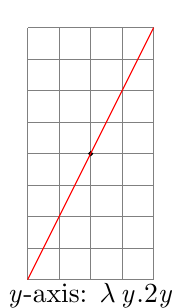
\begin{tikzpicture}[scale=.4]
      \useasboundingbox (-2,-4) rectangle (2,4);
      \draw[very thin,color=gray] (-2,-4) grid (2,4);
      \node[draw,circle,inner sep=.5pt,fill] at (0,0) {};
      \draw[color=red,domain=-2:2] plot (\x,2*\x);
      %% \node[rotate=90] at (-2.5,0) {$\lambda y.y$};
      \node at (0,-4.5) {$y$-axis: $\lambda y.2y$};
    \end{tikzpicture}
    \hspace{8pt}
    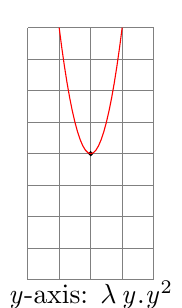
\begin{tikzpicture}[scale=.4]
      \useasboundingbox (-2,-4) rectangle (2,4);
      \draw[very thin,color=gray] (-2,-4) grid (2,4);
      \node[draw,circle,inner sep=.5pt,fill] at (0,0) {};
      \draw[color=red,domain=-1:1] plot (\x,{(2*\x)^2});
      %% \node[rotate=90] at (-2.4,0) {$\lambda y.y^2$};
      \node at (0,-4.5) {$y$-axis: $\lambda y.y^2$};
    \end{tikzpicture}
    \vspace{12pt}
    \caption{lambda x.2x with different y-axis scaling functions.}
    \label{fig:yscaling}
  \end{marginfigure}%

  \newthought{The moral of the story} is that axes, like coordinate
  spaces, are mathematical entities, independent of visual
  representation.  The task of representing the axes of a coordinate
  space is orthogonal to the task of scaling them.  And since we will
  ultimately want a single, unified representation of the composition of
  our stack of coordinate spaces and the figures inscribed in them,
  specifying that representation will be associated with the root
  space.\sidenote{FIXME: elaborate this, or refer to a section that
    does elaborate on cspace composition and specification of axis
    representations.}

  %%%%%%%%
  \subsection{Examples}
  \label{subs:axiseg}


  Cartesian space has x and y axes, each with unit of 1, angle of
  incidence of 0 and 90 deg, respectively, and orientation of x
  increases rightwards, y upwards.

  Example:  parallel axes.  Set y-axis origin to 5, angle of incidence to zero.

  %%%%%%%%%%%%%%%%%%%%%%%%%%%%%%%%
  \section{\CSpace{}s}
  \label{sect:dspaces}

  \begin{remark}
    Take e.g. cartesian and polar as primitive spaces -
    interconvertable, maybe, but having fundamentally different meanings.

    How many primitive spaces are there?
  \end{remark}

  %%%%%%%%
  \subsection{Discrete and Continuous}
  \label{subs:discrcont}

  \begin{remark}
    Discrete spaces = bitmaps.  What to do about functions in a
    discrete \cspace{}?  This is where the concept of ``formula of a
    function'' pays off: we want to use the same formula in both
    cases, but different domains.  Strictly speaking this gives us two
    different functions that happen to share a single formula.  In the
    discrete case we will have to add a domain restriction that
    eliminates all but the integers; fortunately this is easy to
    express in Z: \(\num\dres\real\).

    When we get to curves and figures we will have the task of mapping
  \end{remark}

  %%%%%%%%
  \subsection{Root Set}
  \label{subs:csrootset}

  A \cspace{} is a structure, of which its set of points is just one
  component.  Hence the need to specify the \textit{root set} of
  a \cspace{}.\sidenote{Compare Z, where each type has a carrier set.
    Since a \cspace{} is a type, it has a (Z) carrier set, but that is
    not what the same as its root set.}

  \begin{remark}
    Don't all \cspace{}s have the same root set, namely \Rtwo{}?  (Or
    more generally \(\real ^n\).)  Well, no: the root set of a
    discrete \cspace{} is \(\num ^n\).
  \end{remark}

  %%%%%%%%
  \subsection{Axis Sequence}
  \label{subs:orientation}

  Every \cspace{} is associated with an ordered set of one or more
  axes.  The ordering of this set is critical, because that is what
  determines the interpretation of locative expressions like
  \((a,b)\).

  Axis order is reflected in writing convention: \((a,b)\) just means
  that \(first(a,b)=a\) maps to the first axis (by convention, the $x$
  axis), and \(second(a,b)=b\) maps to the second axis (by convention,
  the $y$ axis).

  \newthought{The orientation of a \cspace{}} determines where points
  \((a,b)\) are positioned relative to the origin.  This depends on the
  \textit{polarity} of the axes--their directions of increasing value--
  and their \textit{order} within the \cspace{}.  By convention, the
  standard cartesian \cspace{} has Q1\sidenote{%
    Q1:  Quadrants are numered counter-clockwise, starting with the upper right quadrant:

    \centering
    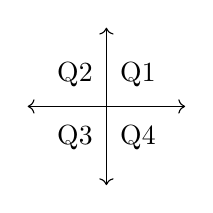
\begin{tikzpicture}[scale=1]
      \useasboundingbox (-1,-1) rectangle (1,1);
      \draw[<->] (-1,0) -- (1,0);
      \draw[<->] (0,-1) -- (0,1);
      \draw (.4,.4) node {Q1};
      \draw (-.4,.4) node {Q2};
      \draw (-.4,-.4) node {Q3};
      \draw (.4,-.4) node {Q4};
    \end{tikzpicture}
  } \((x,y)\) orientation: every point in the first quadrant is
  with first coordinates increasing to the right and second
  coordinates increasing upwards.  To locate a point \((a,b)\) in the
  space, find \(first(a,b)\) on the $x$-axis and \(second(a,b)\) on
  the \(y\)-axis.

  Contrast this with the way cartesian space might be represented in
  cultures with right-to-left writing systems.  For such cultures, it
  would be more ``natural'' -- that is, more consistent with the way the
  writing system organizes space -- to use Q2 \((x,y)\) orientation,
  retaining \((x,y)\) axis order, but reversing the polarity of the
  \(x\) axis.  In Q2, first coordinates%
  \sidenote{%
    \(first(a,b)=a,\ second(a,b)=b\)
  }% would increase to the left rather than the right, placing (+,+)
  %% (+,+)\sidenote{(+,+) \(\rightarrow\) positive in both coordinates}
  points in the second quadrant.  Since the order of the axes remains
  \((x,y)\), that this system is the mirror image of the standard
  cartesian space across the (vertical) y axis.

  \newthought{Changing the axis order} from \((x,y)\) to \((y,x)\) may
  be unorthodox, but it has its uses.  In particular, in typesetting we
  may want to make our \cspace{}s agree with the way writing systems
  organize space.  This means that for some text objects we might want
  to use a \((y,x)\) order.

  For example, both left-to-right and right-to-left writing systems use
  the lower quadrants to organize their writing systems.  Left to right
  systems like English use Q4 orientations: characters flow left to
  right, and lines break, then stack from top to bottom.  Right to left
  systems like Arabic and Hebrew, by contrast, use Q3 orientation: as in
  Q4 left-to-right systems, lines stack top to bottom, but character
  flow (x axis polarity) is reversed, so characters move right to left.

  In both cases, we might want to use a \cspace{} with \((x,y)\) order
  for character layout but one with \((y,x)\) order for line
  layout.\marginnote{TODO: graphic illustration}

  A number of writing systems influenced by the Chinese literary
  tradition have historically organized their texts using a different Q3
  orientation: characters in a line descend top to bottom, and lines in
  a paragraph march from right to left.  For positioning characters, we
  might want to use \((y,x)\) order, so that increasing first
  coordinates track character flow (and thus eye movement) from top to
  bottom.  On the other hand, for positioning lines we might want to use
  \((x,y)\) order, so that increasing first coordinates track line
  stacking leftwards.

  \newthought{The upshot of all this} is that \cspace{}s are somewhat
  more than mere geometry.  They are not just there to make
  transformations of figures possible; they represent ways of organizing
  space.  Organizing space is not a matter of mere geometry; it has
  genuine cultural significance.\sidenote{TODO: something about the
    history of perspective drawing as a way of organizing space and how
    it changed our ways of thinking.  Maybe something from Bachelard's
    Poetics of Space?}

  %%%%%%%%%%%%%%%%
  \section{Transforms}
  \label{sect:transforms}

  \begin{remark}
    \cspace{} transforms are really just the axes as functions.  We should probably eliminate the term.
  \end{remark}

  \begin{remark}
    The interpretation of function application as expressing a
    relation, mentioned in the intro, is critical in treating
    transformations.  Or at least in working with intuitions about
    transformations, as reflected in common CS design patterns.
  \end{remark}

  %%%%%%%%
  \subsection{Coordinate Point Transforms}

  %%%%%%%%
  \subsection{\CSpace Transforms}

  %%%%%%%%
  \subsection{\DSpace Transforms}
  \label{subs:}

  \Cspace{} transform, plus transform of ``lambda points''.  If lambda points are stored as lambda expressions, this amounts to function composition.

  %%%%%%%%
  \subsection{Notes}

  An example will expose the distinction.  Most graphics languages have
  a "transform" function that allows the user to translate, scale,
  rotate, or skew figures.  The syntax usually makes it look like the
  figures are being transformed; e.g.

  let c = (0,0) circle (1)  ;; figure: unit circle at origin
  translate(c, (1,1))	      ;; move origin of circle to (1,1)

  But that is the wrong interpretation; what gets transformed is the
  entire coordinate space in terms of which the figure is directly
  expressed.  We need a vocabulary that allows us to express this
  explicitly.  In the example, we want a way to say explicitly that the
  transform operator applies to a CS, not to a figure.  For example (toy syntax):

  1)	  let origin(cs:$\Omega$) = origin(cs:Root) + (1,1)  ;; start by specifying translation of cs:$\Omega$
  2)	  let c = (0,0) circle (1) in cs:$\Omega$  ;; then specify figure relative to cs:$\Omega$
  3)	  result: unit circle located at (1,1) in cs:Root

  A more succinct (possible) notation, using [ ] to indicate a cs "context" :

  1)	  let cs:$\Omega$[(0,0)] = cs:Root[(0,0)] + (1,1)  ;; origin in $\Omega$ coords = (1,1) in Abs coords
  2)	  cs:$\Omega$[(0,0) circle 1]   ;; circle expressed in cs:$\Omega$ coordinates
  3)	  result: unit circle located at (1,1) in cs:Root

  This may get the idea across, but the problem is that the transform
  expression only specifies the translation of a single point; it does
  not explicitly say that the entire cs is transformed.  A
  transformation is a function, but 2) does not clearly express this.

  CS transformations are functions and should be expressed as such.

  We could associate transformations with the axes of a CS.  For
  example, for cs:Cartesian we might write:

  axis : {name="x", unit=1, transform=\(\lambda x.x\), incidence=0}
  axis : {name="y", unit=1, transform=\(\lambda y.y\), incidence=0}

  But where do the inputs to the transform functions come from, and what
  is the meaning of their outputs?  The basic idea of a transform is
  that it maps points in one CS to points in another CS.  But the
  definition of an axis is scoped its CS, which leaves open the question
  of where we find the xs and ys to which the transforms apply.

  The solution to this problem is to see that transformations are not
  associated with particular spaces.  They map one space to another,
  both of which are in themselves independent of the transformation.  So
  we do not want to include a transformation function as part of the
  definition of a CS.  It's tempting to do so (possibly because of the
  influence of Object-Oriented thinking), but incorrect; a
  transformation is just a function, and is not connected with any
  "class" or "object".  This will lead us below to consider an algebra
  of coordinate spaces.

  It follows that we have to define a default "scale" for each axis,
  just as we define a default unit of 1.  Axiomatically, as it were.

  In other words, it is not accurate to say that transforms "change"
  coordinate spaces.  Instead, they map all the coordinates from one
  space to another, leaving both spaces per se unchanged.  This is
  critical, since it allows us to express various figures, each in its
  own cs, and then map them to a single "parent" cs under different
  transforms.  If transforms had the effect of producing a "distorted"
  version of the source space, this would not be possible, or at least
  it would be much more awkward.

  So how should we express such transformations?  First, since they are
  functions, we can use lambda notation to express them.  E.g.

  {\setstretch{1.25}
    \begin{alignat}{1}
      & \lambda x.x \\
      & \lambda x.2x   ;; scale x axis by factor of 2 \\
      & \lambda x.ln x ;; logarithmic x axis
    \end{alignat}
  }

  Second, we should make explicit the fact that inputs are coordinates
  in one space, and outputs are coordinates in another:

  $$x_a = \lambda x_b.x_b  ;; where _a = cs:Root, _b = cs:\Omega$$

  In other words, we need a typed lambda calculus.

  Third, they are applied to cspaces, but not part of their definitions.
  So:

  \begin{equation}
    x:B["x"] = \lambda a::A["x"].2a
  \end{equation}


  where foo::Bar["baz"] means foo is a coordinate on the "baz" axis of space Bar.

  (This notation is awkward, but at this point we are interested in
  clarity and explicitness.)

  Whatever sort of notation we come up with, we still have the problem
  of how to express the idea that one space is to be mapped into another
  ("into" literally, points into space) /under/ a transformation
  function.  In other words, in addition to specifying the function
  (possibly as a lambda expression), we also need to express the domain
  and range.

  Maybe something like the following, which apes y=f(x) notation:

  cs:B.x = f(cs:A.x)

  But y=f(x) defines a function; it does not explicitly state dom and ran.

  To be really explicit we might try:

  $$f = \lambda x.2x$$

  $$dom(f) = cs:\Omega$$

  $$ran(f) = cs:Root$$

  This has the virtue of clarity.  But each figure in a composition has
  its own "home" cspace, which we call $\Omega$, so we may end up with lots
  of $\Omega$s.  This would leave us to define f for each pair of spaces,
  even if they use the same function.  E.g.


  $$f = \lambda x.2x$$
  dom(f) = cs:\Omega.x, ran(f) = cs:Root.x
  ... draw some stuff into cs:\Omega
  dom(f) = cs:Gamma.x, ran(f) = cs:Root.x
  ... draw some stuff into cs:Gamma

  Here we use two spaces to draw stuff, but map them both to the same
  space using the same transformation.

  Advantage of lambda notation: much easier to express complex
  transformations.  Although vector/matrix notation is pretty handy.

  With lambda we don't need predefined functions like "translate",
  "scale", etc.  (Same is true of vector/matrix notation.)

  With lambda we also get non-linear transformations, e.g.
  \(f = \lambda x.x^2\)

  So a key design decision: how to express transformation functions.
  lambda or matrix?

  Another key design decision: how to express the dom and ran of
  transformation functions.

  [We seem to be approaching something like the standard notion of
    layers.  But with the notion of cspace, we don't need layers.  Or
    rather, layering is a separate idea, which corresponds to order of
    composition.  We can think of cs:$\Omega$ as the top of a stack of
    cspaces, i.e. last (first) in a series of transforms, but we can use
    the same cspace in multiple stacks.]

  ================

  Transform functions v. positioning functions

  Both kinds are total functions; the difference is in how they are
  used.  Transform functions are to be applied to entire coordinate
  systems, mapping every point.  Positioning functions are just like
  transforms, but are intended to be used on subsets of the space,
  esp. on single points in path expressions.

  Some of TikZ's coordinate systems effectively function as positioning functions.

  ================

  Scales

  Note that some transform functions, e.g. scaling, can be applied to
  anything, not just axes.  For example, color gradients, color maps
  (see pgfplots).  So cspaces and axes and ink (styles) are all
  distinct, but transform functions can apply across the board.


  %% ``In the Cartesian plane the point (x, y) can also be represented in polar coordinates as

  %% (x, y) = (r\cos\theta, r\sin\theta)\qquad(r, \theta) = \left(\sqrt{x^2+y^2}, \quad \arctan\frac{y}{x}\right).'' http://en.wikipedia.org/wiki/Complex_plane

  %%%%%%%%%%%%%%%%%%%%%%%%%%%%%%%%
  \section{Canvases}
  \label{sect:canvas}

  \begin{remark}
    A canvas is a space together with an empirical unit of measure,
    e.g. 1cm.  So unlike a \cspace{}, a canvas is not an abstract,
    purely mathematical object.\marginnote{TODO: how does TikZ handle
      the distinction?}

    Another perspective: a \cspace{} has a mathematical but not an
    empirical denotation;\sidenote{Except perhaps space itself} a canvas
    has both.  A canvas represents some physical surface, albeit
    abstractly, whereas a \cspace{} represents
    nothing.\marginnote{Caveat: we're talking about mathematical enties,
      not expressions in a languge.  Of course, a \cspace{}
      \textit{expressions} represents something, namely a \cspace{}; but
      the space itself, as a mathematical ``object'', does not
      represent.}
  \end{remark}

  In a \cspace{}, a point expression \ab{} denotes a \textit{position} in
  a structure; in a canvas, the same expression denotes a
  \textit{location} in (physical) space.\marginnote[-24pt]{Convention:
    positions are structural, locations spatial.}

  Numbers ``in'' a \cspace{} just \textit{are} structural positions;
  ``on'' a canvas, they represent spatial
  location.\marginnote[-12pt]{``Space'' and ``spatial'' are ambiguous
    here. etc.  We should probably refer to coordinate structures rather
    than \cspace{}s.}

  Specifying a point on a canvas is analogous to dabbing a bit of paint
  on a literal canvas.  Specifying a point in a \cspace{} is better
  thought of as analogous to memorizing how to get to a place in a city
  - five blocks west and two blocks north of the
  Courthouse.\marginnote{Recall that numbers can be thought of as
    methods or arcs, rather than objects.}


  %%%%%%%%%%%%%%%%%%%%%%%%%%%%%%%%%%%%%%%%%%%%%%%%%%%%%%%%%%%%%%%%
  %%%%%%%%%%%%%%%%%%%%%%%%%%%%%%%%%%%%%%%%%%%%%%%%%%%%%%%%%%%%%%%%
  \part{Designs}
  \label{part:designs}

  %% %%%%%%%%%%%%%%%%%%%%%%%%%%%%%%%%%%%%%%%%%%%%%%%%%%%%%%%%%%%%%%%%
  %% \part{Curves}
  %% %% \part{Operations on \DSpace{}s}

  %%%%%%%%%%%%%%%%%%%%%%%%%%%%%%%%
  \section{Overview}
  \label{sect:designoverview}


  %%%%%%%%
  \subsection{Compositional Pathways}
  \label{subs:compospath}

  Terminology:
  \begin{description}
  \item [inscription] of a function in a \cspace{}
  \item [image] of a function under another function (syn: graph?)
  \end{description}


  \begin{remark}
    A/K/A ``graphics pipeline''
  \end{remark}


  \[Function \fun Graph \fun Curve \fun Figure \fun Bitmap \fun Ink \]

  \begin{remark}
    This is best viewed in terms of composition of functions, rather
    than sequencing of operations.  So maybe ``pipleline'' is not the
    best metaphor, insofar as it suggests the latter.  ``Stack''?
    ``Journey''?  ``Path''?
  \end{remark}


  %%%%%%%%%%%%%%%%%%%%%%%%%%%%%%%%
  \section{Graphs}
  \label{sect:graphs}

  \begin{remark}
    Move the math bits (definitions) of this to
    \hyperref[sect:thirtysix]{Thirty-six Views}.  Leave only what is
    directly connected with \cspace{} stuff.
  \end{remark}

  A graph is a set of points.  Informally, we might make a distinction
  between the graph of a function and the sort of graph we might
  specify by enumerating its points.  This corresponds to the
  difference between intensional and extensional definitions of sets:
  an intensional definition states a function that serves as a
  membership test to determine which points are members of the set; an
  extensional definition just lists each point explicitly.

  For example, consider the even integers from \(1\) to \(10\).  We
  can express this set extensionally by enumerating its elements: \(E
  = \{2,4,6,8,10\}\).  To express the same set intensionally, we use
  \hyperref[subs:setcomp]{set comprehension notation}: \(\{\forall
  i:\nat | i\in [1\upto 10] \land \exists n | i = 2n @ i \}\)

  But the difference is only apparent; an extensional definition of a
  set of points whose first elements contain no repetitions is by
  definition the definition of a function.  So we can always think of
  any graph as the graph of some function.

  \begin{remark}
    Is this true?  Important?  What do we gain (or lose) by thinking
    of every graph as the graph of some function?  Does having two
    kinds of graph - those produced by functions and those not,
    intensional and extensional - cause any problems?
  \end{remark}

  \begin{remark}
    What about circles, rectangles, and other figures whose graphs are
    not in fact functions?  We can express them parametrically.
  \end{remark}

  {\todo In any case, the purpose of this section is not just to
    define ``graph'' but to examine the various ways available for
    expressing graphs using Z.}

  A graph is not yet a curve or figure; as a mere set of ordered pairs
  of numbers, a graph has no intrinsic connection with a
  particular \cspace{} and thus no antecedently determined visual
  representation.  It all depends on the \cspace{} and its transforms:
  the same graph can take on a very different appearance in different
  spaces.  The graph of a straight line, for example, doesn't look
  very straight when plotted in a polar \cspace{}.  To get from graph
  to image, we have to bind the graph to a definite \cspace{}.  When
  we do this, we end up with a \textit{curve}, which is the
  \textit{image of the graph under the \cspace{}}.  Curves are
  discussed in the next section.

  \begin{remark}
    Can we always rewrite an extensional definition of a set
    intensionally?  At a minimum, we can use the identity function
    together with an enumeration of its domain.  For example, instead
    of writing \[S=\{ (0,0), (3,7), (28,195)\}\] we can write ...
  \end{remark}

  %%%%%%%%%%%%%%%%%%%%%%%%%%%%%%%%
  \section{Curves}
  \label{sect:figs}

  A curve is the image of a graph under a \cspace{}.  Informally, this
  means we obtain a curve by applying the axial transformation
  functions of the \cspace{} to each point of a graph, yielding the
  image of the graph (i.e. a set of points) ``in'' the \cspace{}.

  \begin{remark}
    Critical point: conceptually the pipeline from function to graph
    to curve to figure can be thought of as just transformations of
    sets of points, and thus a sequence of sets; this is the Z
    perspective.  But that might not be very helpful for implementors;
    you can't store an infinite set of points in a computer.  So it is
    better to take a more lambda-oriented perspective, and think in
    terms of a composition of functions.  You cannot store the graph
    of a function in a computer, but you can store (a representation
    of) the lambda term expressing the function, which you can later
    use to find a subset of its graph.
  \end{remark}

  \begin{remark}
    Figure as sequence v. figure as set.  This parallels function as
    operation v. function as set of ordered pairs.  Or lambda
    expressions v. their reductions.  Sort of.

    Every sequence can be ``reduced'' (projected?) to a set.  So we
    can model any figure as a set of points in a space.  But if we
    want to support e.g. path operations that depend on a ``current
    point'', then we need to model figures as sequences, which will
    give us operators like ``first'' and ``last''.

  \end{remark}

  %%%%%%%%%%%%%%%%%%%%%%%%%%%%%%%%
  \section{Figures}
  \label{sect:figures}

  %% \part{Figures}
  %% \label{sect:representation}

  \begin{remark}
    Two topics:
    \begin{itemize}
    \item How to visually represent mathematical \cspace{}s
    \item How to use \cspace{}s (and their visual representations) to
      represent the real world (or possible worlds) (as with e.g. OpenGL coord. spaces).
    \end{itemize}
  \end{remark}

  A figure is the image of a curve under an \textit{inking} function.
  Inking functions map points to sets of points representing geometric
  figures and associate each point with a color (ink).

  Informally, the way to make a curve visible is to map each of its
  points to a ``micro-figure'' consisting of the points of a geometric
  form such as a circle and associate a color with each point in the
  result.  So a line can be made visible by ``drawing'' a black circle
  around each of its points; this would result in the appearance of a
  solid line whose height is equal to the diameter of the circles
  around its points, and whose ends are rounded.  To get a line with
  square ends, draw a square instead of a circle around each of its
  points.


  %%%%%%%%
  \subsection{Point Expressions}
  \label{subs:pointexprs}

  \ab as expression - denotes a pair of reals (type \RR), not a point in
  a \cspace{}.  Note: \RR is a type expression, not a cs.  If we want to
  think of \RR as \Rtwo space, then it must be a (or: the one and only)
  absolute space, with axiomatically defined axes, etc.  A \ab
  expression outside of an cs context does not denote a coordinate
  point.  Inside a cs context, it denotes a pair in \RR (\Rtwo) which
  the cs scaling functions map to a point in the \Rtwo associated with
  the cs.  (CS a combo of \Rtwo, axes, etc.)

  So it is incorrect to think of a cs only in terms of \Rtwo.  It's a
  different mathematical structure.

  A pair of reals \ab only becomes a ``point'' when interpreted ``by'' a
  cs, mapping from pure \Rtwo to a cs structure - which we can think of
  as a mapping from pure number ``location''.

  %%%%%%%%
  \subsection{Space Expressions}
  \label{subs:spaceexprs}

  %%%%%%%%
  \subsection{Figure Expressions}
  \label{subs:figexprs}

  %% %%%%%%%%%%%%%%%%%%%%%%%%%%%%%%%%%%%%%%%%%%%%%%%%%%%%%%%%%%%%%%%%
  %% \part{Ink}
  %% \label{part:ink}

  %%%%%%%%%%%%%%%%%%%%%%%%%%%%%%%%
  \section{Ink}
  \label{sect:}

  \begin{remark}
    This should be in another paper, it isn't really about \cspace{}s.
  \end{remark}

  %%%%%%%%%%%%%%%%%%%%%%%%%%%%%%%%
  \subsection{Color}
  \label{sect:color}

  %%%%%%%%%%%%%%%%%%%%%%%%%%%%%%%%
  \subsection{Pattern}
  \label{sect:pattern}

  %%%%%%%%%%%%%%%%%%%%%%%%%%%%%%%%
  \subsection{Gradient}
  \label{sect:gradient}

  %%%%%%%%
  \subsection{Transparency}
  \label{subs:transparency}

  %%%%%%%%%%%%%%%%%%%%%%%%%%%%%%%%
  \section{Misc}
  \label{sect:}

  %%%%%%%%
  \subsection{\DSpace{}s}
  \label{sect:dspaces}

  \begin{remark}
    Do we really need a distinct type?  Can't we just augment \Omg?
  \end{remark}

  \begin{remark}
    Structure, then functions.
  \end{remark}

  %%%%%%%%
  \subsection{Design Points}
  \label{sect:dpts}

  \begin{remark}
    What to call points ``inscribed'' into a \cspace{}?  Addresses?
    Locations?  Pixels?  Such points ``look like'' coordinate points,
    but they are not literall ``in'' the \cspace{}; rather they are
    ``stored'' in a separate structure, so the \cspace{} and the list
    of ``design points'' together make up a compound structure.  It is
    only when the time comes to actually ink a surface - a page or
    screen - that they get mapped to some location ``in'' (rather,
    ``on'') something.  Locatives denote locations?  Mention v. use;
    ``\((a,b)\)'' v. \((a,b)\)
  \end{remark}

  \begin{remark}
    We use the term \textit{lambda point} to refer to points that have
    been ``added'' to \cspace{}s, in order to distinguish between points
    that are present in the \cspace{} by definition and points that are
    added (inserted, projected, etc.) ``into'' the space.  So if we draw
    a point at \origin{} into space \Omg{}, the result is a space that
    contains the same \origin{} point it had to start with, plus the
    lambda point we projected on to that ``native'' point.
  \end{remark}

  \begin{remark}
    Lambda pt as func application - lambda expr, plus arg.
  \end{remark}

  Suppose we start with \cspace{} \Omg{}, and we define a point \ab ``in''
  \Omg{}; something like

  \begin{equation}
    \label{eq:omgapplic}
    Let\ C_1 = \Omega[(a,b)]
  \end{equation}

  Then we transform \Omg{} into some other \cspace{}--call it \(\Gamma\),
  by writing something like

  \begin{equation}
    \label{eq:gammapplic}
    Let\ C_2 = \Gamma[C_1]
  \end{equation}

  The question we want to address now is: what happens when we do this?
  What do statements like these (and their component expressions)
  denote?  What precisely do expressions like \(\Omega[(a,b)]\) and
  \(\Gamma[C_1]\) mean? What do \(C_1\) and \(C_2\) ``contain''?  What
  happened to \ab in formula \ref{eq:gammapplic}?

  Let's start by asking what \Omg{} denotes before we ``apply'' it to a
  \hyperref[subs:pointexprs]{point expression}.  According to our definitions, a \cspace{} denotes
  the combination of:

  \begin{itemize}
  \item \(\mathds{R}\times\mathds{R}\)\marginnote{\(\mathds{R}\times\mathds{R}\)
    = the set of all ordered pairs of real numbers, i.e. Points.}
  \item A pair of axis definitions, each including a scaling function.
  \item A specification of axis order.
  \end{itemize}

  Specifically, let's assume that \Omg{} denotes the \sccs{}; then it
  has \(x\) and \(y\) axes, ordered \xy{}, that have

  \begin{itemize}
  \item Angles of incidence \(0\degree\) and \(90\degree\), respectively
  \item Default (positive) polarity
  \item Identity scaling functions (\(\lambda x.x\))
  \end{itemize}

  So far so good.  Now what does \(Let\ C_1=\Omega[(a,b)]\)
  mean?  Specifically, that is; what's the machinery?

  \begin{remark}
    Long story short: applying a \cspace{} to a point yields a pair of
    the original \cspace{} and a representation of the point.  Under
    eager evaluation, that representation is of the form
    \ab\marginnote{\ab: TODO explain why this should still be considered
      a lambda expression.}; under lazy evaluation, it is the
    (unevaluated) lamba form expressing applyication of the axis scaling
    functions to the coordinates of the point.

    In other words, \cspace{}s never change (immutability); they just
    carry the points they contain along with them as a list of (lambda)
    expressions; hence ``lambda points''.  Only on the last step of
    transforming the design space to device space are all the forms
    fully evaluated.
  \end{remark}

  %%%%%%%%
  \subsection{Ink}
  \label{subs:ink}

  a/k/a style or graphics state

  %%%%%%%%
  \subsection{\DSpace{} Application}
  \label{subs:dsapplic}

  A \dspace{} is formally defined as a function.  This allows us to
  express what traditional languages usually call
  \textit{transformations} as function applications.

  \begin{gendef}[X,Y]
    \_[\_] : \Delta\cross\Delta\fun\Delta \\
    \_[\_] : \Gamma\cross\Gamma\fun\Gamma \\
    \where

  \end{gendef}

  A \textit{\dspace{} application} maps one \dspace to another \dspace{}.



  %%%%%%%%%%%%%%%%%%%%%%%%%%%%%%%%%%%%%%%%%%%%%%%%%%%%%%%%%%%%%%%%
  %%%%%%%%%%%%%%%%%%%%%%%%%%%%%%%%%%%%%%%%%%%%%%%%%%%%%%%%%%%%%%%%
  \part{Content}
  \label{part:content}

  \begin{remark}
    This goes in a separate paper, not directly relevant to \cspace{}s.
  \end{remark}

  %%%%%%%%%%%%%%%%%%%%%%%%%%%%%%%%
  \section{Connecting Content to Graphs}
  \label{sect:geomcontent}

  ================

  For browsers (rather, XML structures), treat the DOM as coordinate
  space?

  ================

  D3 first "selects" DOM nodes, then brings in the data.  That seems
  backwards.  First read the data, then project to the design space.

  ================

  The DOM+CSS model.  Boxes (some of them, anyway) implicitly define
  coordinate systems.  Adding an element - a paragraph, say - to the DOM
  does two things: it inserts a node into the (abstract) tree, and it
  maps the new node to a figure located in a coordinate space.  So to
  the hierarchy of the DOM corresponds a hierarchy of cspaces.
  Ultimately constrained by the display device.

  What about adding an svg circle (d3 examples)?  The svg cspace gets
  inserted into the cspace of the doc.  So there is an implicit
  transform mapping coords from the cs:SVG to cs:DOM. Or rather than
  cs:DOM, to whatever cspace is associated with the DOM parent of the
  svg node.  Call it the "host" cspace?  In any case, this is all
  implicit.

  A DOM node always has an associated piece of geometry.  Compare TikZ
  nodes, which are named bits of geometry.

  Note that you cannot transform a cspace you are attaching to the DOM;
  attaching always means mapping origin to origin. (?)  You can
  transform subspaces within the cs:SVG, but you cannot use any
  transform other than the identity transform for mapping cs:SVG to
  cs:Host.

  Weeell, not really; you can use CSS positioning and offsetting.  So
  you can specify a transform, but not directly as a transform.  That's
  one of the design shortcomings of CSS.

  Plus, you rarely know where a host node cspace is itself going to end
  up after composition.

  In any case, the goal pursued here is investigation of DOM as a kind
  of coordinate space.  Or more generally (covering XML as well as
  HTML), of tree structured data and their relation of graphic
  coordinate spaces.


  ================

  Kinds of "content coordinate spaces".  Sequence, Relation, Tree, Graph
  (net).

  Plaintext is a sequential structure, so display of plaintext editor
  maps sequence to one cspace.

  Postscript has some hierarchy - pages, for example.  But basically the
  graphical figs on a postscript page do not map to a tree structure.
  You can reference variables, data structures, etc. within PS, but
  that's all internal.  There is no content data structure that stands
  separate from the language, as is the case with XML, where there is a
  data structure and API used by client languages.

  PDF?  Another page description language; I don't recall much of a
  content model standing separate from the graphic language, but it's
  been quite a while since I looked.

  In all these cases, when you add a figure to a space, you say where it
  is to be placed.  You might express that in terms of offsets or
  something, but you always refer to some known point of reference.  You
  don't just say "offset (x,y) from the upleft corner of parent
  figure, wherever that happens to end up" as is the case with HTML+CSS.

  Hmm.  Better review my PS/PDF.  As in most graphics languages, when
  you position something at (x,y) in PS/PDF, the implicit assumption is
  that the cspace involved may be transformed later.  So all positioning
  is relative until demonstrated otherwise.

  So what are we looking for here?  Uniformity of expression?  We want
  to use the same positioning language for both web and print targets.
  In particular, we want to completely hide the DOM, since a DOM API
  would be meaningless for e.g. PDF.  The D3 strategy of "selecting" DOM
  nodes and then binding data makes no sense if there is no DOM.

  A graphics language just specifies graphicky stuff, not content stuff.
  D3 and similar muddies the distinction by mingling content access
  vocab and graphics vocab.

  One approach: treat DOM nodes (and selectors) as names of coordinates
  in cspace.  Compare named nodes in TikZ/PGF.  Then the semantics would
  be purely geometric.  At least for accessing; what about
  adding/appending?  Appending a DOM node corresponds to specifying
  another point in cspace.  Think path v. ink.  Appending an empty div
  node is just like adding a point object to the path collection.  The
  difference is that the cs coords of the empty div are unresolved; it's
  like saying "add a point object, but I'll tell you the coordinates
  later".  In other words, like an unevaluated lambda(?), or a "virtual"
  point.  Another diff: DOM objects inherently ordered; add two empty
  divs and they will retain that order.  Add two virtual points and they
  are unordered.  Or: the only order in a cspace is that defined by the
  geometry of the space.  The temporal order in which stuff gets added
  is discarded.

  Or: the order of an XML tree is just abstract order, A precedes B,
  without any concrete definition of what "precedes" means (i.e. it does
  not mean greater than, less than, etc.)

  %%%%%%%%%%%%%%%%%%%%%%%%%%%%%%%%
  \section{Caveats}
  \label{sect:caveats}

  Beware of people who contrast ``logical'' and ... something else.  For
  example, the Unicode folks contrast ``logical order'' and ``visual
  order''
  (\url{http://userguide.icu-project.org/transforms/bidi#TOC-Logical-Order-versus-Visual-Order}).  Some people refer to ``logical dimensions'' and ``display dimension'' in HTML5.

  %%%%%%%%%%%%%%%%%%%%%%%%%%%%%%%%%%%%%%%%%%%%%%%%%%%%%%%%%%%%%%%%
  \part{Notes}

  %%%%%%%%%%%%%%%%%%%%%%%%%%%%%%%%
  \section{Algebra of Coordinate Spaces}
  \label{sect:csalgebra}


  In addition to origin and axes, coordinate systems always have an
  algebra, which specifies operations on coordinate points.  This allows
  us to distinguish between e.g. cartesian and complex cspaces.

  Cartesian:

  \begin{itemize}
  \item +  =  scale unit of source arithmetically; e.g. cs:A[(0,0)]+(1,1)
  \item *  =  scale unit of source geometrically: (x,y)*(a,b) = (ax,by) e.g. cs:A[(1,1)]*(2,2)
  \item ?  =  rotation
  \item ?  =  skew (shear)
  \item ?  =  reflection
  \item ?  =  glide reflection (http://en.wikipedia.org/wiki/Transformation\_(function))
  \end{itemize}

  NB: "scale" usually means scale multiplicatively, but it applies
  equally to arithmetic transformation.  We can talk of arithmetic,
  geometric, harmonic, etc. scaling.

  Complex:

  * = (x+yi)*(a+bi) = (xa - yb) + (xb + ya)i

  (x,y)*(a,b)   = ((xa-yb), (xb+ya))

  e.g. (1,0)(0,1) = ((0-0), (1+0)) = (0,1) = i
  ================

  %%%%%%%%%%%%%%%%%%%%%%%%%%%%%%%%
  \section{Primitive Coordinate Spaces}
  \label{sect:primitives}

  \begin{remark}
    Only one truly primitive, axiomatic space: cartesian?  All the
    others can be transformed into plain cartesian space.  But for
    practical reasons we will include some predefined spaces that will
    count as primitive in our language, even if they are not
    mathematically primitive.  Primitive expressivity, as it were.
  \end{remark}

  Affine:  "In mathematics, an affine coordinate system is a coordinate system on an affine space where each coordinate is an affine map to the number line. In other words, it is an injective affine map from an affine space A to the coordinate space Kn, where K is the field of scalars, for example, the real numbers R.  The most important case of affine coordinates in Euclidean spaces is real-valued Cartesian coordinate system. Orthogonal affine coordinate systems are rectangular, and others are referred to as oblique." (http://en.wikipedia.org/wiki/Affine\_coordinates)

  Homogenous:  "In mathematics, homogeneous coordinates or projective coordinates, introduced by August Ferdinand Mobius in his 1827 work Der barycentrische Calcul,[1][2] are a system of coordinates used in projective geometry, as Cartesian coordinates are used in Euclidean geometry. They have the advantage that the coordinates of points, including points at infinity, can be represented using finite coordinates. Formulas involving homogeneous coordinates are often simpler and more symmetric than their Cartesian counterpart." (http://en.wikipedia.org/wiki/Homogeneous\_coordinates)

  \begin{itemize}
  \item Cartesian  (logarithmic a special case?)
  \item Polar
  \item Complex
  \item Cylindrical
  \item Spherical
  \item Log-polar
  \end{itemize}

  ================


  Primitive cspaces always same, alterations come via transforms.
  Untransformed, the default is just plain Cartesian space, unit=1,
  scale is identity func, incidence 0 and 90, orientation standard.

  But what about polar space?  We can transform a cartesian space into a
  polar space, but we cannot draw directly into a polar space using
  cartesian coordinates.  So we need polar space as a primitive space.
  Two axes: angular (length along circumference) and radial (length of
  vector).

  %%%%%%%%%%%%%%%%%%%%%%%%%%%%%%%%
  \section{Misc}
  \label{sect:misc}

  Drawing a figure always involves two specifications, one explicit, the
  other (usually) implicit.  The explicit specification describes the
  figure: size, shape, location\sidenote{Design space includes a style
    element involving color, line thickness, etc. but we can ignore that
    for present purposes.}.  The implicit specification describes the
  coordinate space.  The explicit specification (of a figure) is always
  relative to a coordinate space.

  CS (Coordinate Space) specification:  origin (always 0) + axes


  Example: unit circle centered at the origin.  The usual way to specify
  this is something like

  (0,0 circle(1)  (using tikz syntax; any other would do as well)

  This is the explicit specification; implicit is the specification of the CS.

  \begin{remark}
    The idea is that expressions like \((a,b)\) find a first home in the
    Root space, which is standard, absolute, Cartesian space.  You
    cannot ``touch'' Root space; its fixed.  But you can ``insert''
    things into Root design space, and you can apply transforms to it to
    yield other spaces.
  \end{remark}

  But there are always two coordinate spaces: the one in which
  coordinates are directly expressed (as above), which we'll call the
  Root space, and the "\Omg" space to which the Root space is mapped.
  In other words, specifying a figure and a space is not enough; the
  space itself must be located in a "parent" space, which we're calling
  the \Omg space.  Maybe Alpha space would be better.\marginnote{Since
    Alpha is beginning and Omega is end; we begin by specifying points
    in absolute space, map spaces to spaces, and end up in device space
    (=\Omg space).}

  [Root space is axiomatic: x and y axes with unit = 1, incidence 0 and
    90, the usual orientation.  Root space is also absolute.]

  IOW, the minimal transform is the \(Ident\) transform, which maps the
  Root space directly to \Omg space with no changes.  Expressions in
  which a transform is not explicitly specified always implicitly use
  the \(Ident\) transform.

  \begin{remark}
    All spaces are immutable; all we can do is express mappings between spaces.
  \end{remark}

  [NB this is all device independent.  Mapping root space to device
    space is a separate issue.]

  [NB third kind of space, between device independent (abstract) root
    space and device space: device-independent space with empirical units
    of measure.  E.g. x and y axes with unit = 1cm (instead of just 1).]

  \clearpage
  %%%%%%%%%%%%%%%%%%%%%%%%%%%%%%%%%%%%%%%%%%%%%%%%%%%%%%%%%%%%%%%%
  \part{Appendices}
  %% \appendix
  %% \appendixpage
  \begin{appendices}
    %%%%%%%%%%%%%%%%%%%%%%%%%%%%%%%%
    \section{Formal Definitions}
    \label{sect:formadefs}

    %%%%%%%%
    \subsection{Generalized Application Operators}
    \label{subs:genappop}

    \marginnote{\textbf{Caveat:} We cheat a little bit here and there.
      For example, Z does not allow operator overloading (to my
      knowledge, anyway).  These definitions would fail if run through
      an automated Z specification checker; however, our main purpose
      here is expressive, so we don't care.  At the moment, we just
      want our definitions to be clear, complete, and unambiguous for
      the human reader.}

    These operators generalize function application to the case of
    applying a function across a bounded domain.  It is critically
    important to understand that these are just functions with special
    notation.\sidenote{We could have used standard notation, something
      like ``\(graphproj(a,b,f)\)'' instead of
      \(\displaystyle\sideset{_a}{^b}{\bigg|}f\), but the latter seems
      much clearer; its form conveys information.  The former might be
      a good email syntax, but where reasonably good typesetting
      facilities are available the latter notation seems clearly
      preferable.} In fact, like the famous ``map, filter, reduce''
    troika, these are second-order functions -- functions that operate
    on other functions.

    \begin{remark}
      Realized belatedly that Z is already equipped with an operator
      that makes this trivial: domain restriction.  \([a\upto b]\dres
      f\) denotes precisely what we want: the graph of a function over
      an interval.  But still the vertical bar notation is useful to
      have.
    \end{remark}

    \vspace{6pt}
    \noindent
    %%%%%%%%%%%%%%%%
        {\defn Domain Projection}

        \begin{gendef}[X,Y]
          \sideset{_{\strut\_}^{\strut\_}}{}{\bigg|}\_ : X\cross X\cross(X\fun Y)\fun \power X \\
          \where
          \forall a,b : X, f : X\fun Y| \forall x:X | x\in [a\ldots b]\ \exists y:Y|f(x)=y @ \{x\}
        \end{gendef}

        Domain projection of a function over an interval just returns the
        set of elements of the domain of application for which \(f\) is
        defined.  Less formally:
        \[\displaystyle\sideset{_a^b}{}{\bigg|} f(x) = \{\forall z:\real | z\in [a..b] @ z\}\]

        \vspace{6pt}
        %%%%%%%%%%%%%%%%
        \noindent
            {\defn Range Projection}

            \begin{gendef}[X,Y]
              \sideset{}{_{\strut\_}^{\strut\_}}{\bigg|}\_ : X\cross X\cross(X\fun Y)\fun \power Y \\
              \where
              \forall a,b : X, f : X\fun Y| \forall x:X | x\in [a\ldots b]\ \exists y:Y|f(x)=y @ \{f(x)\}
              %% \forall f : X\fun Y, \forall x : X | x\in [a\ldots b], \exists y | f(x)=y @ \{f(x)\}
            \end{gendef}

            Range projection of a function over an interval applies the
            function to every element \(x\) of the domain of application for
            which it is defined and returns the union of the results \(f(x)\)
            as a set.  Less formally:

            \[\displaystyle\sideset{}{_a^b}{\bigg|} f(x) = \{\forall z:\real | z\in [a..b] @ f(z)\}\]

            \vspace{6pt}
            \noindent
                {\defn Graph Projection}

                \begin{gendef}[X,Y]
                  \sideset{_{\strut\_}}{^{\strut\_}}{\bigg|}\_ : X\cross X\cross(X\fun Y)\fun \power (X\cross Y)
                  \where
                  \forall a,b : X, f : X\fun Y| \forall x:X | x\in [a\ldots b]\ \exists y:Y|f(x)=y @ \{(x,f(x))\}
                  %% \forall f : X\fun Y, \forall x : X | x\in [a\ldots b],\exists y|f(x)=y @ \{(x,f(x))\}
                \end{gendef}

                Graph projection of a function over an interval applies the
                function to every element \(x\) of the domain of application for
                which it is defined, forms the ordered pair \((x,f(x))\), and
                returns the union of the results as a set of ordered pairs.  Less
                formally:

                \[\displaystyle\sideset{_a}{^b}{\bigg|} f(x) = \{\forall z:\real | z\in [a..b] @ (z, f(z))\}\]

                \begin{commentary}
                  We could have defined these operators to work only for functions
                  defined on the entire interval.  However, our main concern is
                  with graphics languages, not mathematics per se, so we will
                  sometimes want to graph functions over intervals that may
                  contain ``bad'' elements.  For example, \(\lambda x.1/x\) is
                  undefined at \(0\), but we may want to graph it over the
                  interval \([-1\ldots 1]\).  So a better solution is to restrict
                  the domain to those values for which the function is defined;
                  that is what the clause ``(\(\exists y|f(x)=y\))'' does.  So in
                  this example, the result will effectively omit \(0\) from the
                  domain before applying the function.  This is good enough for
                  generating a visual representation of the function.

                  \emph{Reminder:} these definitions are not intended as
                  programming models.  In real-world graphics DSLs, plotting of
                  functions involves sampling the specified domain, usually at a
                  user-specified frequency.  In addition, many function values may
                  be far outside the range that can be shown on a piece of paper
                  or a screen; for example, values of \(\frac{1}{x}\) close to
                  zero.  Implementations may handle this situation in a variety of
                  ways.  But for the purpose of formally defining the logic and
                  mathematics of graphics languages we don't need to worry about
                  such stuff - we can and must leave such implementation details
                  to language designers and programmers.  (NB: we're not designing
                  a programming language here, we're extending a specification
                  notation.)
                \end{commentary}

                \begin{eg} Graph of \(\frac{1}{x}\) over the half-open interval
                  \((0\ldots 1]\): \(\sideset{_{(0}}{^{1]}}{\bigg|}\lambda x.\frac{1}{x} \)
                \end{eg}

                %%%%%%%%
                \subsection{Coordinate}
                \label{subs:coorddefn}

                \[COORD == \real\]

                %%%%%%%%
                \subsection{Angle}
                \label{subs:angledefn}

                \[RADIAN == \real\]

                \[DEGREE == \real\]

                \begin{axdef}
                  degToRad : \real\fun\real \\
                  radToDeg : \real\fun\real
                  \where
                  \forall x : \real @ degToRad(x) = x\cdot\frac{\pi}{180} \\
                          {\small\strut} \\
                          \forall x : \real @ radToDeg(x) = x\cdot\frac{180}{\pi}
                \end{axdef}

                %%%%%%%%
                \subsection{Point}
                \label{subs:pointdefn}

                \[POINT == COORD\cross COORD \]

                %%%%%%%%
                \subsection{Identity Function}
                \label{subs:idfndefn}

                \begin{gendef}[X]
                  ident : X\fun X
                  \where
                  \forall x : X @ ident(x) = x
                \end{gendef}

                %%%%%%%%
                \subsection{Axis}
                \label{subs:axisdefn}

                An \textit{axis} is ...\marginnote{Do we need to explicitly list the carrier set (\R)?}

                \begin{schema}{Axis}
                  origin : COORD \\
                  offset : COORD \\
                  incidence : RADIAN \\
                  scale : COORD\fun COORD
                  \where
                  origin = (0,0) \\
                  offset = scale(origin)
                \end{schema}

                %%%%%%%%
                \subsection{\CSpace}
                \label{subs:csdefn}

                A \textit{\cspace} combines \RR{} and a sequence of axes.\marginnote{Do we need to explicitly list the carrier set (\Rtwo)?}

                %%%%%%%%
                \subsection{\DSpace}
                \label{subs:dspacedefn}

                A \textit{\dspace} is a \cspace{} plus a set of figures.

                %%%%%%%%
                \subsection{Curve}
                \label{subs:curvedefn}

                A curve is a set of points, that is, a graph.  We call it a curve
                rather than a graph in order to stress the point that a curve
                represents a spatial interpretation to the graph.

                The symbol for the curve of a function over a range is \(Big|_a^b f\).

                The advantage of having a specific curve operator is that it
                allows us to concisely and clearly indicate the end points of a
                curve.  Most function symbols do not provide such a convenience;
                prominent exceptions are the summation sign \(\Sigma_a^b\) and the
                integral sign \(\int_a^b\).  But to indicate the graph (curve) of
                \(f\) from \(a\) to \(b\), some ad-hoc technique must be found,
                e.g. \(f(x),\ x\in [0..1]\).  With \(\Big|_a^b\) we can just write:

                \[\bigg|_a^b \lambda x.2x \]

                Why do we need this?  Aside from convenience and expressivity?
                It allows us to specify figures (plotted functions)
                in \dspace{}s.  For example, the line segment from the origin
                to \((1,1)\):

                \[\bigg|_0^1 \lambda x.x\]

                This gives us a concise notation that we can use to provide a
                concise formal definition of e.g. TikZ's path operators like
                ``--'', rectangle, etc.

                It will also help us express transform composition clearly; without
                it that would be difficult.

                \begin{remark}
                  TODO: write formal Z definition of this operator.
                \end{remark}


                %%%%%%%%
                \subsection{Path}
                \label{subs:pathdefn}

                A path is a function; it denotes a curve.  Techically, a path denotes
                its graph.

                %%%%%%%%%%%%%%%%%%%%%%%%%%%%%%%%
                \section{Previous Work}
                \label{sect:prevwork}

                \epigraph{Immature poets imitate; mature poets steal}{TS Eliot}


                %%%%%%%%
                \subsection{\TeX, \MF, and \MP}

                %%%%%%%%
                \subsection{TikZ/PGF}
                \label{subsec:tikz}

                TikZ has by far the most sophisticated concept of coordinate space.

                Canvas =  x,y with explicit "dimension" (empirical UOM)

                XYZ    =  x,y,z as "factors" multiplying unit vectors of length 1cm)

                Canvas Polar = radius expressed in canvas system, i.e. with UOM

                XYZ Polar  = radius and angle interpreted in as in xy csystem, i.e. factors (of unit vectors of 1cm) not dimensions

                XY Polar (=XYZ Polar)

                Barycentric  -  "In geometry, the barycentric coordinate system is a coordinate system in which the location of a point of a simplex (a triangle, tetrahedron, etc.) is specified as the center of mass, or barycenter, of masses placed at its vertices. Coordinates also extend outside the simplex, where one or more coordinates become negative."   (http://en.wikipedia.org/wiki/Barycentric\_coordinate\_system)

                Node (=DOM?)  The cs:node is parasitic the more primitive empirical
                systems.  It allows you to refer to a previously specified point by
                specifying its name and an "anchor" or predefined location relative to
                the node's position.  The anchor name effectively denotes a function
                that computes a point, given the node' base point.

                Tangent Like cs:node, cs:tangent supports specification of points by
                refering to previously specified points.  A tangent function is
                implicitly applied to the points refered to - actually a point and a
                figure - and computes the tangent from the point to the figure.

                Custom -- the job of a custom cs is to compute x and y in the canvas
                coordinate system.  So defining a custom coordinate system boils down
                to specifying a transformation function.

                TikZ's XYZ system behaves like an abstract Euclidean system.  But it
                does have default unit vectors that map it to canvas space.

                \begin{remark}
                  Compare Asymptote.  TikZ systems that allow unitless coordinate
                  specifications (e.g. XYZ) use an implicit empirical UOM (default:
                  1cm).  Any \cspace{} must eventually be mapped to a canvas.
                \end{remark}

                Thus all TikZ cspaces are empirical; some seem to provide means of
                expressing coordinates rather than establishing a distinct system;
                e.g. node and tangent systems.  They don't (at least not all of them)
                establish a primitive interpretation of (x,y).  For example, the
                tangent cs does not provide a meaning for any (x,y); instead, it
                allows you to specify a (tangent) point by reference to an already
                specified pair of a shape and a point.

                In other words, cs:node and cs:tangent are derived systems, the others
                primitive.  They are essentially transform functions using for
                positioning.  They do not need units of measure since that is already
                implicit in the points they reference.  Dunno about barycentric, which
                I don't really grok yet.

                Basically all the cspaces amount to positioning functions, which is
                why they can be mixed in single path expressions.

                Correction: they are NOT transform functions, in that they do not
                transform the entire csystem; instead they are positioning functions,
                designed to transform subsets of the space.

                Furthermore, TikZ's system allows for use of multiple coord systems in
                one expression.  So you can write (0,0) -- (polar cs:
                cs:angle=90,radius=1cm), using first the xyz (Id func) system then the
                polar system (a positioning function) to draw a line from the origin
                to (0,1), unit=cm.

                Note that the xyz cs seems to be the default for (x,y) syntax, where x
                and y are dimensionless.

                %%%%%%%%
                \subsection{Postscript}

                Figure specification as executable program.

                User space, device space

                Units

                %%%%%%%%
                \subsection{PDF}

                Ref:  PDF32000-1:2008 (\url{http://www.adobe.com/devnet/pdf/pdf\_reference.html}

                ``canvas''

                ``[A] PDF content stream is not a program to be interpreted; rather, it is a static description of a sequence of graphics objects.'' p.110

                Five ``graphics objects'': path, text, external, inline image, shading

                Add: clipping path

                ``A shading object describes a geometric shape whose colour is an arbitrary function of position within the shape. (A shading can also be treated as a colour when painting other graphics objects; it is not considered to be a separate graphics object in that case.)'' (p. 111)


                8.3 Coordinate Systems (p. 114)

                ``Coordinate systems define the canvas on which all painting occurs.'' (p.114)

                ``A coordinate space is determined by the following properties with respect to the current page:
                • The location of the origin
                • The orientation of the x and y axes
                • The lengths of the units along each axis'' p.114

                Device space

                User space
                ``Coordinates in user space (as in any other coordinate space) may be specified as either integers or real numbers, and the unit size in default user space does not constrain positions to any arbitrary grid. The resolution of coordinates in user space is not related in any way to the resolution of pixels in device space.'' p.115

                Transforms: translation, scaling, rotation, skewing


                ``The transformation from user space to device space is defined by the current transformation matrix (CTM), an element of the PDF graphics state...'' p.116

                Other coordinate spaces: text space (w/text matrix), glyph space
                (w/font matrix), image space (w/out transforms), form space (matrix),
                pattern space (matrix), 3D stuff

                See figure 12, p. 117

                %%%%%%%%
                \subsection{CSS}

                \url{http://www.w3.org/TR/CSS2/box.html}

                \href{http://www.w3.org/TR/CSS2/visuren.html}{Visual Formatting Model}

                \href{http://www.w3.org/TR/CSS2/visuren.html#containing-block}{Containing
                  Block} ``In CSS 2.1, many box positions and sizes are calculated
                with respect to the edges of a rectangular box called a containing
                block. In general, generated boxes act as containing blocks for
                descendant boxes; we say that a box "establishes" the containing block
                for its descendants. The phrase "a box's containing block" means "the
                containing block in which the box lives," not the one it
                generates....Each box is given a position with respect to its
                containing block, but it is not confined by this containing block; it
                may overflow.''

                So the ``containing block'' is both geometric and structure.  CSS
                generally maps geometric structure to content structure directly.

                \href{http://www.w3.org/TR/CSS2/visuren.html#normal-flow}{9.4 Normal Flow}

                CSS \href{http://www.w3.org/TR/CSS2/media.html}{media types}; \href{http://www.w3.org/TR/css-print/}{CSS Print Profile}

                \href{http://www.w3.org/TR/css3-page/}{CSS Paged Media Module Level 3}

                \href{http://www.w3.org/TR/css3-page/#page-model}{The Page Model}

                %%%%%%%%
                \subsection{SVG}

                \url{http://www.w3.org/TR/SVG11/coords.html}

                Viewport space, user spaces

                %%%%%%%%
                \subsection{HTML5 Canvas}
                \label{subs:html5}

                \url{http://www.whatwg.org/specs/web-apps/current-work/multipage/the-canvas-element.html}

                ``The canvas element provides scripts with a resolution-dependent bitmap canvas, which can be used for rendering graphs, game graphics, art, or other visual images on the fly.'' \url{http://www.w3.org/TR/html5/scripting-1.html#the-canvas-element}

                ``The CanvasRenderingContext2D 2D rendering context represents a flat linear Cartesian surface whose origin (0,0) is at the top left corner, with the coordinate space having x values increasing when going right, and y values increasing when going down. The x-coordinate of the right-most edge is equal to the width of the rendering context's scratch bitmap in CSS pixels; similarly, the y-coordinate of the bottom-most edge is equal to the height of the rendering context's scratch bitmap in CSS pixels.

                The size of the coordinate space does not necessarily represent the size of the actual bitmaps that the user agent will use internally or during rendering. On high-definition displays, for instance, the user agent may internally use bitmaps with two device pixels per unit in the coordinate space, so that the rendering remains at high quality throughout. Anti-aliasing can similarly be implemented using over-sampling with bitmaps of a higher resolution than the final image on the display.''\url{http://www.whatwg.org/specs/web-apps/current-work/multipage/the-canvas-element.html}

                \url{http://diveintohtml5.info/canvas.html}

                \href{https://developer.apple.com/library/safari/documentation/AudioVideo/Conceptual/HTML-canvas-guide/Introduction/Introduction.html#//apple_ref/doc/uid/TP40010542-CH1-SW1}{Safari HTML5 Canvas Guide}

                ``The canvas is a two-dimensional grid. The coordinate (0, 0) is at the upper-left corner of the canvas. Along the X-axis, values increase towards the right edge of the canvas. Along the Y-axis, values increase towards the bottom edge of the canvas.'' (\url{http://diveintohtml5.info/canvas.html})

                Each canvas element has a ``drawing context''.

                ``One of the most exciting features of HTML5 is the <canvas> element that can be used to draw vector graphics...'' \url{http://www.1stwebdesigner.com/design/creative-ways-use-html5-canvas/}


                \href{http://msdn.microsoft.com/en-us/hh534406.aspx}{The Developer’s Guide to HTML5 Canvas}

                \href{http://msdn.microsoft.com/en-us/library/ff975057.aspx}{CanvasRenderingContext2D object} - methods and props

                ``To draw on a canvas, you need to reference the context of the canvas.  The context gives you access to the 2D properties and methods that allow you to draw and manipulate images on a canvas element.'' \url{http://msdn.microsoft.com/en-us/hh534406.aspx}

                ``everything in the canvas is a pixel.'' http://msdn.microsoft.com/en-us/hh534406.aspx

                ``The canvas 2D API is an object that allows you to draw and
                manipulate images and graphics on a canvas element.  To reference the context of the canvas, you call getContext, which is a method on the canvas element.  It has one parameter, which currently is 2d.  Here’s the snippet of code for referencing the context.

                ``Each canvas has its own context, so if you’re page contains multiple canvas elements; you must have a reference to each individual context that you want to work with.'' \url{Canvas 2D
                  API}  Correction: not an ``object'', a mathematical structure.

                \href{http://blogs.msdn.com/b/ie/archive/2011/04/22/thoughts-on-when-to-use-canvas-and-svg.aspx}{Thoughts on when to use Canvas and SVG}

                %%%%%%%%
                \subsection{OpenGL}
                \label{subs:opengl}


                \href{http://www.matrix44.net/cms/notes/opengl-3d-graphics/coordinate-systems-in-opengl}{Coordinate Systems in OpenGL}

                ``There are multiple coordinate Systems involved in 3D Graphics:

                Object Space
                World Space (aka Model Space)
                Camera Space (aka Eye Space or View Space)
                Screen Space (aka Clip Space)''

                \url{http://www.cse.ohio-state.edu/~parent/classes/581/Lectures/4.2DviewingHandout.pdf}

                %%%%%%%%
                \subsection{OS X/iOS Drawing}

                \href{https://developer.apple.com/library/mac/documentation/graphicsimaging/conceptual/drawingwithquartz2d/dq\_overview/dq\_overview.html}{Quartz 2D}

                \href{https://developer.apple.com/library/mac/documentation/graphicsimaging/conceptual/drawingwithquartz2d/dq\_overview/dq\_overview.html#//apple\_ref/doc/uid/TP30001066-CH202-CJBBAEEC}{Quartz 2D Coordinate Systems}

                Cocoa (OS X):  \url{https://developer.apple.com/library/mac/documentation/cocoa/conceptual/CocoaDrawingGuide/Transforms/Transforms.html#//apple\_ref/doc/uid/TP40003290-CH204-BCIDJJBI}

                iOS:  ??

                %%%%%%%%
                \subsection{Android Drawing}

                \href{http://developer.android.com/guide/topics/graphics/2d-graphics.html}{Canvas and Drawables}

                Transform operators are in the API ref, but the dev guides don't say much about it.

                %%%%%%%%
                \subsection{Direct3D, Direct2D}
                \label{subs:direct3d}


                \href{http://msdn.microsoft.com/en-us/library/dd370990%28VS.85%29.aspx}{Direct2D}

                  \href{http://msdn.microsoft.com/en-us/library/dd756655(v=vs.85).aspx#the_direct2d_coordinate_space}{The Direct2D Coordinate Space}

                  \href{http://msdn.microsoft.com/en-us/library/windows/desktop/ff476345(v=vs.85).aspx}{Programming Guide for Direct3D}

                  \href{http://msdn.microsoft.com/en-us/library/windows/desktop/bb324489(v=vs.85).aspx}{3D coordinate systems and geometry}

                  %%%%%%%%
                  \subsection{R}
                  \label{subs:r}

                  Each ``plotting region'' has its own coordinate space.

                  %%%%%%%%
                  \subsection{Octave}
                  \label{subs:octave}

                  Graphic objects: figure, axes, line, text, patch, surface, text and image.

                  %%%%%%%%%%%%%%%%%%%%%%%%%%%%%%%%
                  \section{Bibliography}
                  \label{sect:bib}

                  %% \addcontentsline{toc}{chapter}{Bibliography}
                  \bibliography{space.bib% don't omit the %!
                    %% ../bib/logic.bib%
                    %% ,../bib/math.bib%
                    %% ,../bib/stats.bib%
                  }
                  \bibliographystyle{plainnat}
                  %% \printbibliography[heading=none]
  \end{appendices}

\end{document}
